%!TEX TS-program = pdflatex
%!TEX root = i3det-top.tex
%!TEX encoding = UTF-8 Unicode

\section{\label{sect:online}Online Systems}

The IceCube online systems comprise both the software and hardware at the
detector site responsible for data acquisition, event selection,
monitoring, and data storage and movement.  As one of the goals of IceCube
operations is to maximize the fraction of time the detector is sensitive to
neutrino interactions (``uptime''), the online systems are modular so that
failures in one particular component do not necessarily prevent the
continuation of basic data acquisition. Additionally, all systems are
monitored with a combination of custom-designed and industry-standard tools
so that detector operators can be alerted in case of abnormal conditions.

\subsection{\label{sect:online:dataflow}Data Flow Overview}

The online data flow consists of a number of steps of data reduction and
selection in the progression from photon detection in the glacial ice to
candidate physics event selection, along with associated secondary
monitoring and data streams.  An overview of the data flow is shown in
Fig.~\ref{fig:online_dataflow}.

\begin{figure}[!h]
 \centering
 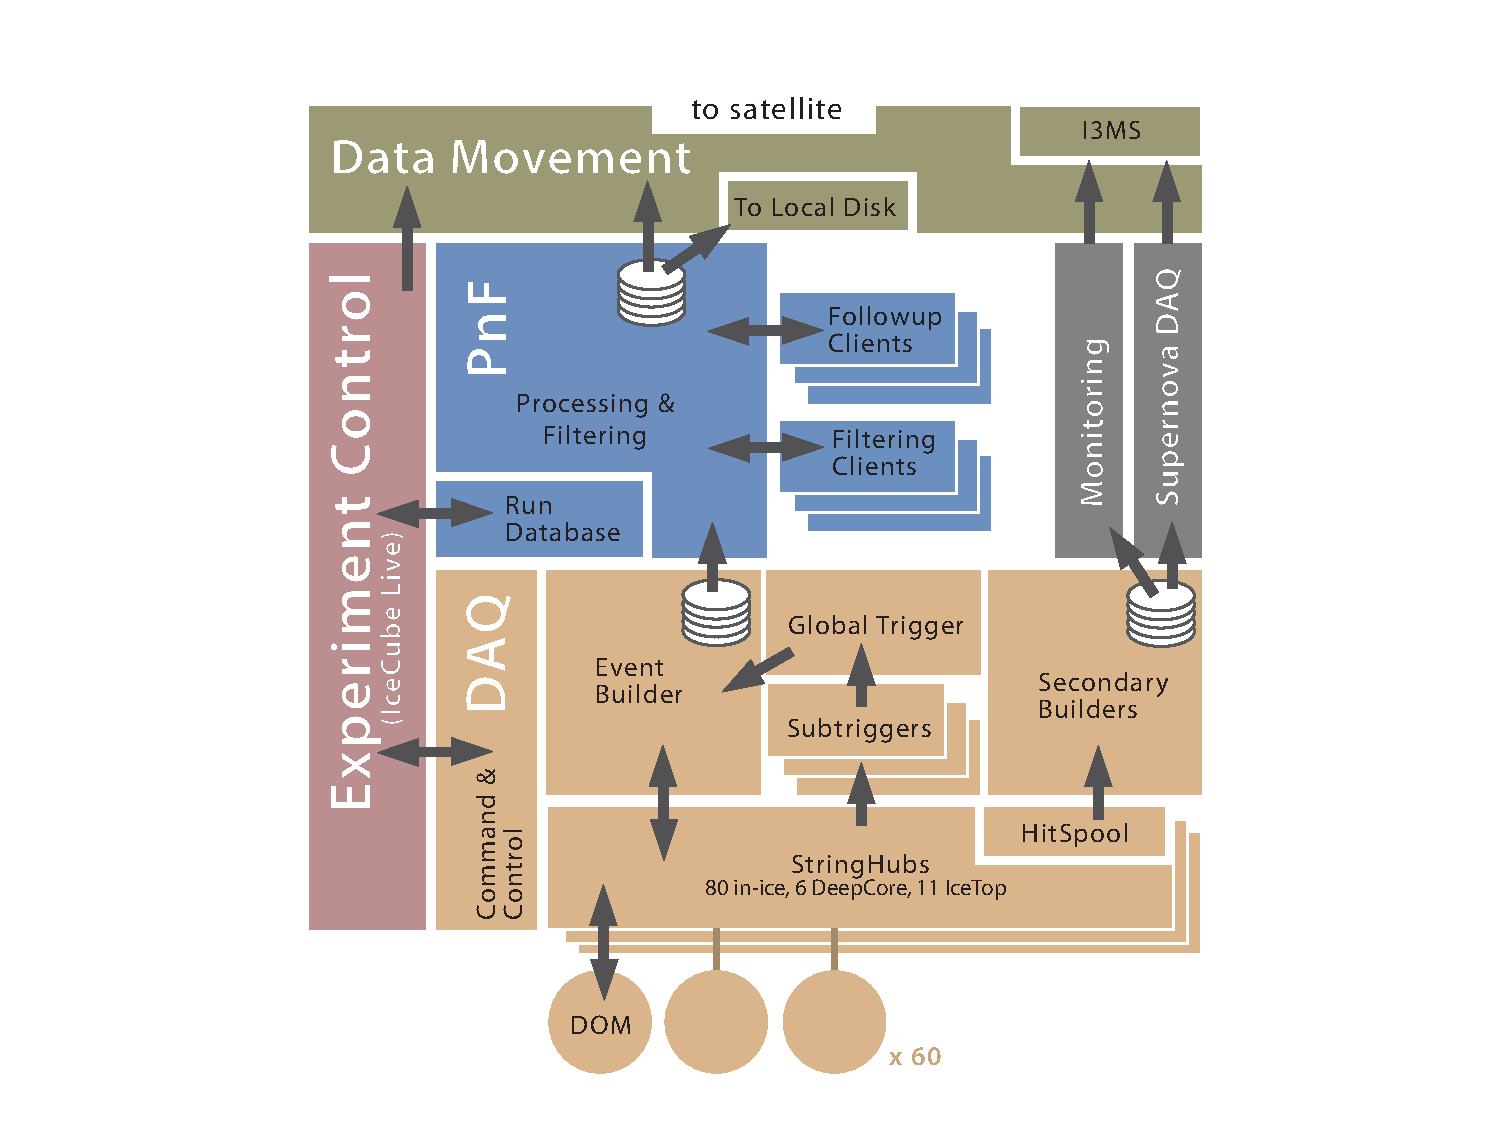
\includegraphics[width=0.6\textwidth]{graphics/online/online_dataflow.pdf}
 \caption{Data flow in the primary IceCube online systems.}
 \label{fig:online_dataflow}
\end{figure}

DOM-level triggers, or hits, are mostly due to dark noise. The first step
in data reduction uses the Local Coincidence (LC) condition described in
Sec.~\ref{sec:dom_functional}.  Hits that meet the LC criteria are flagged
as Hard Local Coincidence (HLC hits) and include a full payload of
digitized waveforms, while isolated non-LC hits are flagged as Soft Local
Coincidence (SLC hits) and are compressed more aggressively.

All DOM hits are read out to dedicated computers on the surface
(Sec.~\ref{sect:sps}) by the data acquisition system (DAQ).  The next level
of data selection is the formation of triggers by the DAQ system
(Sec.~\ref{sect:online:trigger}). HLC hits across the detector are examined
for temporal and in some cases spatial patterns that suggest a common
causal relationship.  A number of different trigger algorithms run in
parallel, described in Sec.~\ref{sect:online:trigger}.  All hits (both HLC
and SLC) within a window around the trigger are combined into events, the
fundamental output of the DAQ, and written to disk.  The event rate varies
seasonally with the atmospheric muon flux from 2.5 to 2.9 kHz,
and the total DAQ data rate is approximately 1~TB/day.

The DAQ also produces secondary streams that include time calibration,
monitoring, and DOM scaler data.  The scaler data, which monitorings the
noise rate of each DOM in 1.6 ms bins, is used in the supernova data
acquisition system (Sec.~\ref{sect:SNDAQ}) to detect a global rise in the
noise rate from many $O(10)$ MeV neutrino interactions occurring in the ice
from a Galactic core-collapse supernova.  The time calibration and
monitoring streams are used to monitor the health and quality of the
data-taking runs.

The DAQ event data is then processed further with a number of filters
in order to select a subset of events (less than 10\%) to transfer over
satellite to the Northern Hemisphere (Sec.~\ref{sect:online:filter}).  Each
filter, typically designed to select events useful for a particular physics
analysis, is run over all events using a computing cluster in the ICL.
Because of limitations both on total computing power and bounds on the
processing time of each event, only fast directional and energy
reconstructions are used.  This Processing and Filtering (PnF) system is
also responsible for applying up-to-date calibration constants to the DAQ
data. All processed events, even those not selected by the online filters,
are stored locally for archival.

A dedicated system for data movement handles the local archival storage to
tape or disk, as well as the handoff of satellite data
(Sec.~\ref{sect:online_jade}).  This includes not only primary data streams
but also monitoring data, calibration runs, and other data streams.

Experiment control and detector monitoring are handled by the IceCube Live
software system, described in Sec.~\ref{sec:online:icecubelive}.

\subsection{\label{sect:sps}SPS and SPTS}

The South Pole System (SPS) comprises 18 racks of computing and network
hardware in the ICL that run the various online systems described in this
section.  The DOM surface cables are connected via passive patch panels to
custom 4U DOMHub computers, one DOMHub per in-ice string and 11 additional
hubs for IceTop.  The remaining servers, including those for higher-level
data acquisition, event filtering, detector monitoring, and core
infrastructure, are currently 2U Dell PowerEdge R720 servers running
Scientific Linux (see Table \ref{tab:sps_breakdown}).  The servers are
typically upgraded every 3 to 4 years.  The custom hardware components in
the DOMHubs are replaced with spares as failures warrant, and the disks and
single-board computer (SBC) were upgraded in 2013--14.

\begin{table}[h]
  \centering
  \begin{tabular}{ r | c }
    \bf{Component} & \bf{\#} \\ \hline DOMHubs & 97 \\ Other data
    acquisition & 4 \\
%    Experiment control & 1 \\
    Monitoring & 3 \\ Event filtering & 24 \\ Infrastructure & 8 \\ Other &
    6 \\
  \end{tabular}
  \caption{Breakdown of computing equipment at SPS, indicating number of
    machines used for each task.}
  \label{tab:sps_breakdown}
\end{table}

The DOMHub is an industrial computer chassis with custom components for DOM
power, timing, and communication.  A low-power single-board computer
communicates with 8 custom PCI DOM Readout (DOR) cards via a PICMG 1.0
backplane.  A dual-redundant ATX power supply powers the DOMHub, while two
48VDC Acopian power supplies, mounted and connected in series inside the
chassis, supply power to the DOMs.  The DOM power is switched and
monitoring by the DOR cards and is controllable by software.  Another PCI
card, the DOMHub Service Board (DSB), is responsible for GPS timing fanout
(Sec.~\ref{sect:online:master_clock}).

The SPS computers are connected via a 48 Gbps switch that in turn fans out
to switches in each DOMHub rack; the DOMHub switches are connected with
dual bonded 10 Gbps links.  The hubs and servers are connected to local
switches with dual bonded 1 Gpbs links.  Typical network I/O during
data-taking for the DAQ event builder (see
Sec.~\ref{sect:online:evbuilder}) is $\sim30$ MBps in each direction, while
the master PnF node sees 25 MBps in and 80 MBps out.

Redundancy and continuous monitoring of SPS is one of the keys to a high
detector livetime.  Nagios monitoring software detects and flags problems,
including issues with DOM power and communication on the hubs.  Severe
problems impacting data-taking result in a page to the IceCube winterover 
personnel via the station's Land Mobile Radio (LMR) system.  A dedicated
hot spare server can replace any failed DAQ node, while spare PnF filtering
clients can be started to increase throughput in case of a data filtering
backlog.  SPS hardware is also connected to dual redundant uninterruptible
power supplies (UPS) in order to continue data-taking through station power
outages of up to 15 minutes.

A scaled-down version of SPS, the South Pole Test System (SPTS) located in
Madison, Wisconsin, U.S.A., allows testing and validation of both hardware
and software in the Northern Hemisphere before rollout to SPS.  Servers and DOMHubs
identical to those at SPS, along with a small number of DOMs in chest
freezers, are used in the test system.  Although the number of DOMs
available is much smaller than in the real detector, recent software
improvements have allowed the ``replay'' of pre-recorded raw SPS hit data
on SPTS systems, providing a data stream to higher-level DAQ and PnF
components identical to SPS.  Another test system includes a full-length
in-ice cable and is used primary for validation of DOM communications and
timing.

\subsection{Data Readout and Timing}

While the low-level communications and timing systems of the DOM are
described in detail in Ref.~\cite{ref:domdaq}, we review those here in the
context of the broader online systems.

\subsubsection{\label{sect:online:comms}Communications}

Digital communication between the DOR card and DOM occurs via copper
twisted pairs, with two DOMs per pair on the in-ice cable, and one IceTop
DOM per pair for increased bandwidth.  The physical layer signaling is via
amplitude shift key (ASK) modulation.  The protocol is a custom
packet-based scheme.  Each packet is assigned a sequence number, and all
received packets are acknowledged if the sequence number is correct.  Each
packet also contains a CRC checksum to detect transmission errors.
Out-of-sequence packets received are ignored, and non-acknowledged packets
are retransmitted.

Messaging is managed from the surface, in that the DOR requests data from
each DOM in turn; only one DOM can transmit at a time.  Communication is
paused every second to perform a timing calibration (RAPCal; see
Sec.~\ref{sect:dom:rapcal})) via reciprocal bimodal pulse transmission to
each DOM; this provides a time-dependent translation of DOM clock to DOR
clock for every module.  The total bandwidth of the communication channel
is 90 kBps per twisted pair.

% Add more details about actual usage?
% Q: is LC signaling documented anywhere yet?  Should it go here?

\subsubsection{\label{sect:online:master_clock}Master Clock System}

The DOR clocks themselves are synchronized to UTC via an active fanout
system from a single Symmetricom ET6000 GPS receiver with a
temperature-stabilized 10 MHz oscillator, also known as the Master Clock.
The 10 MHz output, a 1 Hz (PPS) output, and a serial time string indicating
the UTC date and time are distributed to the DOMHubs via a series of
fanouts, using shielded, delay-matched twisted-pair cables.  Within the
DOMHub, the DSB card continues the fanout via short delay-matched patch
cables to each DOR card.  The local 20 MHz clocks of each DOR card are
phase-locked to the distributed 10 MHz signal.  The fanout tree is shown in
Fig.~\ref{fig:clock_fanout}.

Since the master GPS receiver is a single-point failure for the detector, a
hot spare receiver, using its own GPS antenna and powered through a
dedicated UPS, is continuously active and locked in case of problems with
the primary.

\begin{figure}[!h]
 \centering
 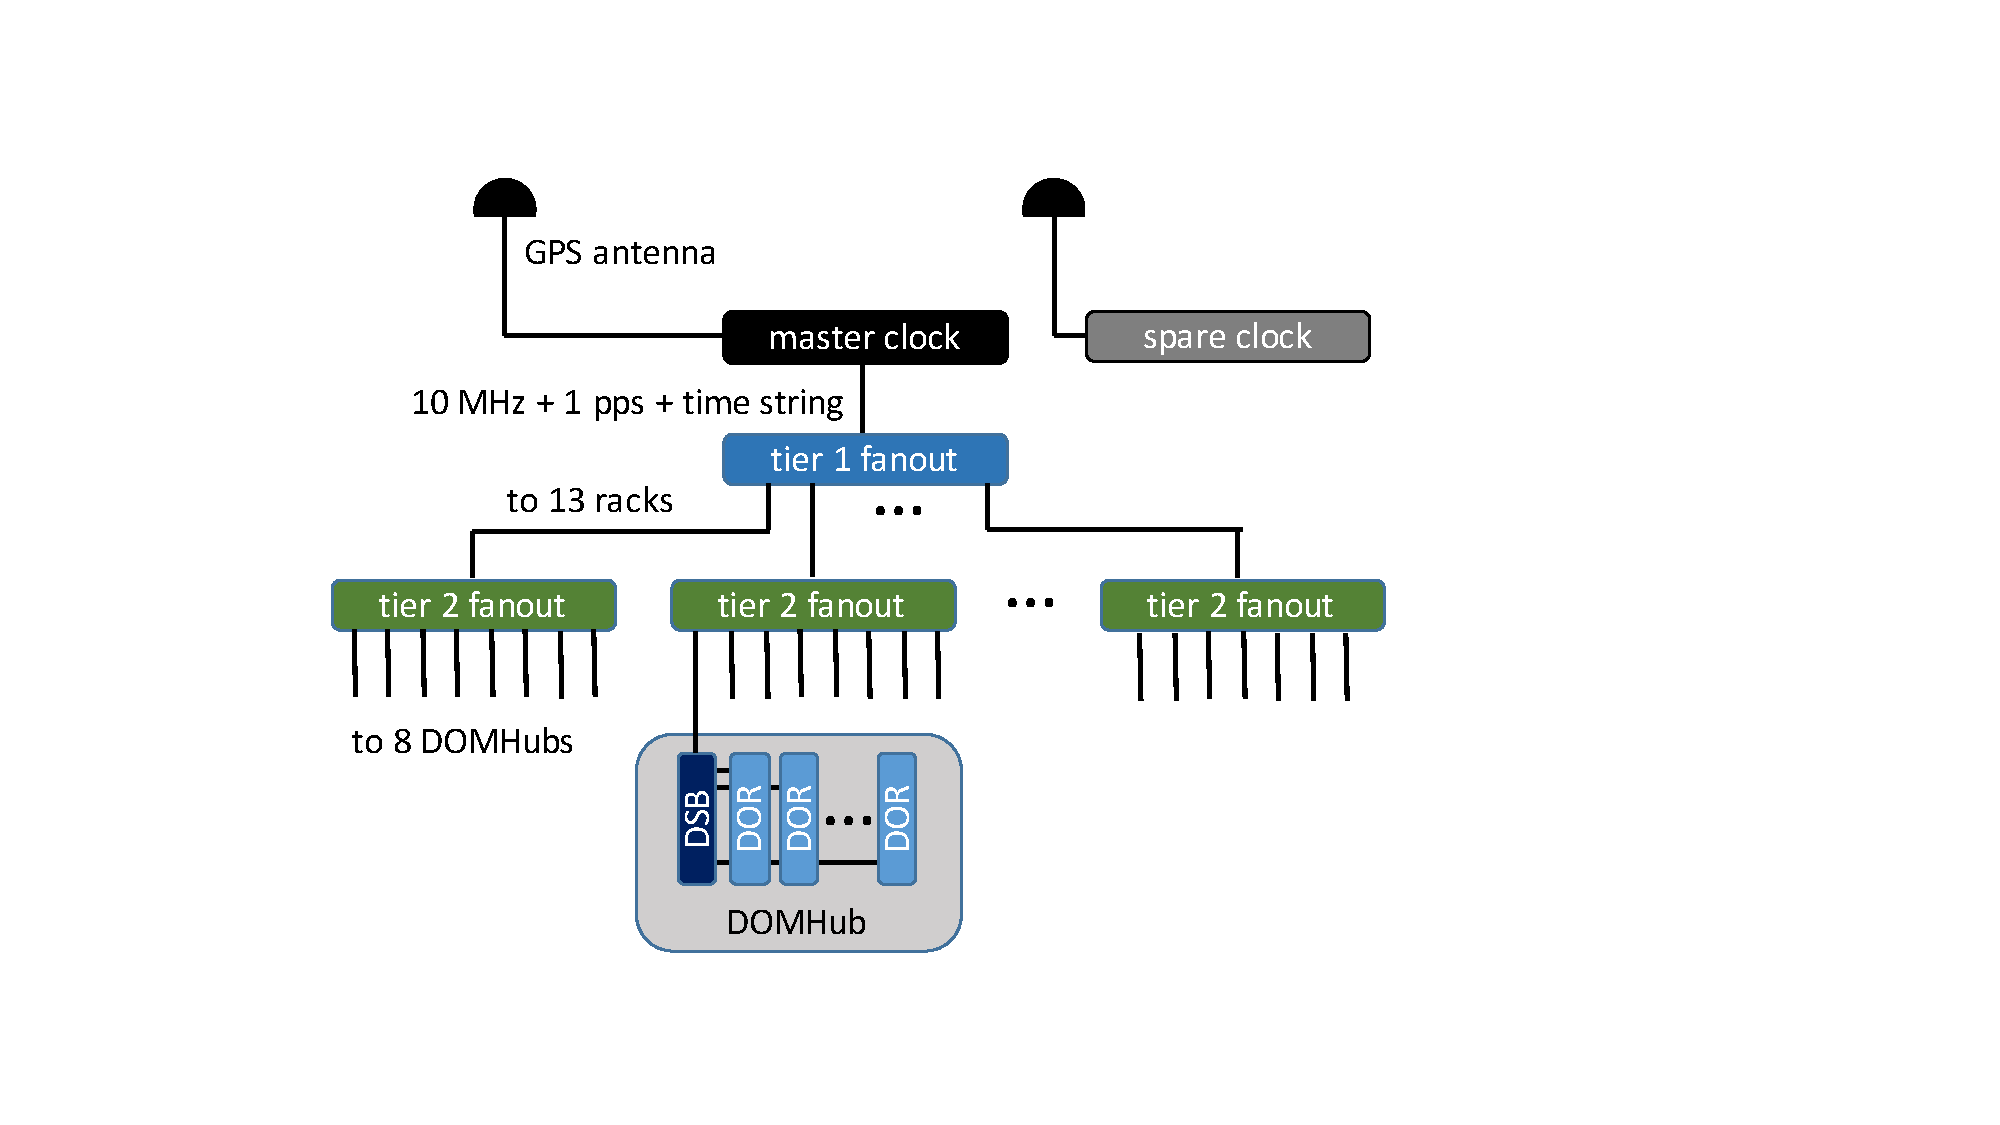
\includegraphics[width=0.8\textwidth]{graphics/online/data_readout/clock_fanout.pdf}
 \caption{Master clock fanout system, from GPS receiver to DOR cards in
   each DOMHub.}
 \label{fig:clock_fanout}
\end{figure}

% Q: do we correct for fanout delay of ~150 ns anywhere?
% Q: say anything about leap seconds?

\subsubsection{DOR Card and Driver}

Each DOR card is connected to up to 8 DOMs, with 8 DOR cards in a
DOMHub. The DOR card controls the 96~V DC power supply to the DOMs and
multiplexes the ASK communications signaling on top of this DC level.
Dedicated circuitry monitors the current draw and voltage levels on each
twisted pair, and in addition to physical fuses, a ``firmware fuse'' can
disable power if the current draw deviates from predefined maximum or
minimum levels.

The software interface to the DOR card, and thus to the DOMs, is provided
with a custom Linux device driver.  Access to DOR card functions, including
DOM power control, communication statistics, RAPCal, current and voltage
monitoring, etc.~is facilitated using the Linux \texttt{/proc} filesystem
interface.  Data transfer from the cards to the single-board computer is
achieved via DMA over the PCI bus.  The driver provides a device file for
each DOM for read/write access by higher-level software.

\subsection{Data Acquisition Software}

IceCube's data acquisition (DAQ) software system is a set of components running on
dedicated servers in the ICL.  Hits are read from the DOMs by the
StringHub components, and a minimal representation of each HLC hit is
forwarded to the ``local'' Trigger components (either in-ice or IceTop.)
The ``local'' Trigger components run these hits through a
configurable set of algorithms and form windows around interesting temporal
and/or spatial patterns.  These time windows are collected by the
``global'' Trigger and used to form non-overlapping trigger requests.
The trigger requests are used by the Event Builder component as templates
to gather the complete hit data from each StringHub and assemble the final
events.

\subsubsection{StringHub and HitSpool}
\label{sec:domhub_hitspool}

The StringHub software component which runs on each DOMHub is responsible
for periodically reading all available data from each of its connected DOMs
and passing that data onto the downstream consumers.  It also saves all
hits to a local ``HitSpool'' disk cache, as well as queuing them in an
in-memory cache to service future requests from the Event Builder for full
waveform data.

The StringHub component is divided into two logical pieces.  The front end,
called Omicron, controls all of the connected DOMs, forwarding any
non-physics data to its downstream consumers and sorting the hits from all
DOMs into a single time-ordered stream before passing them to the back-end
Sender.  The Sender caches SLC and HLC hits in memory, then forwards a
condensed version of each HLC hit to the appropriate local Trigger.

Omicron is also responsible for translating DOM hit times into
UTC-compatible ``DAQ time'', which counts the number of 100-ns periods
since the UTC start of the year (including leap seconds).  The translation
uses the RAPCal procedure as described in Sec.~\ref{sect:dom:rapcal},
performed for each DOM every second. Occasional outliers from the RAPCal
time calibrations are discarded.

%In order to avoid saturating the 2006-era network, the StringHub sends only
%simplified HLC hit data to the local Triggers.  Fields extracted from the
%full HLC are the string and DOM, the time of the hit, and a few DOM trigger
%fields (type, mode, configuration ID), for a total of 38 bytes per hit.

The second, back-end portion of the StringHub component is the Sender.  After the
Trigger components have determined interesting time intervals, 
the Event Builder requests each interval from the Sender which returns a list of
all hits within the interval, pruning all older hits from the in-memory hit
cache after each interval.

One core assumption of the DAQ is that each component operates on a
time-ordered stream of data.  The DAQ uses its ``Splicer'' to accomplish
this.  The Splicer is a common object which gathers all input streams
during the setup phase; no inputs can be added once started.  Each stream
pushes new data onto a ``tail'', and the Splicer merges the data from all
streams into a single sorted output stream.  When a stream is closed, it
pushes an end-of-stream marker onto its tail which causes the Splicer to
ignore all further data.  Details of the Splicer algorithm can be found in
Ref.~\cite{vlvnt13_trigger}.  

% The algorithm at the core of the Splicer is a cascaded binary merge tree.
% The fundamental node consists of two input linked lists (L and R), a
% comparator, and an output linked list (SINK). When an item is pushed into
% the tail of L or R, if the other peer list is non-empty, the lesser of the heads of
% the two lists is pushed into SINK (see Fig.~\ref{fig:hkn1}).  These nodes are
% assembled into a tree, with the top level L/R lists connected to the input
% streams, and the final output SINK providing the merged, sorted stream.
% In this way, pushing into one of the tree inputs ripples through to the output.

% \begin{figure}[!h]
%  \centering
%  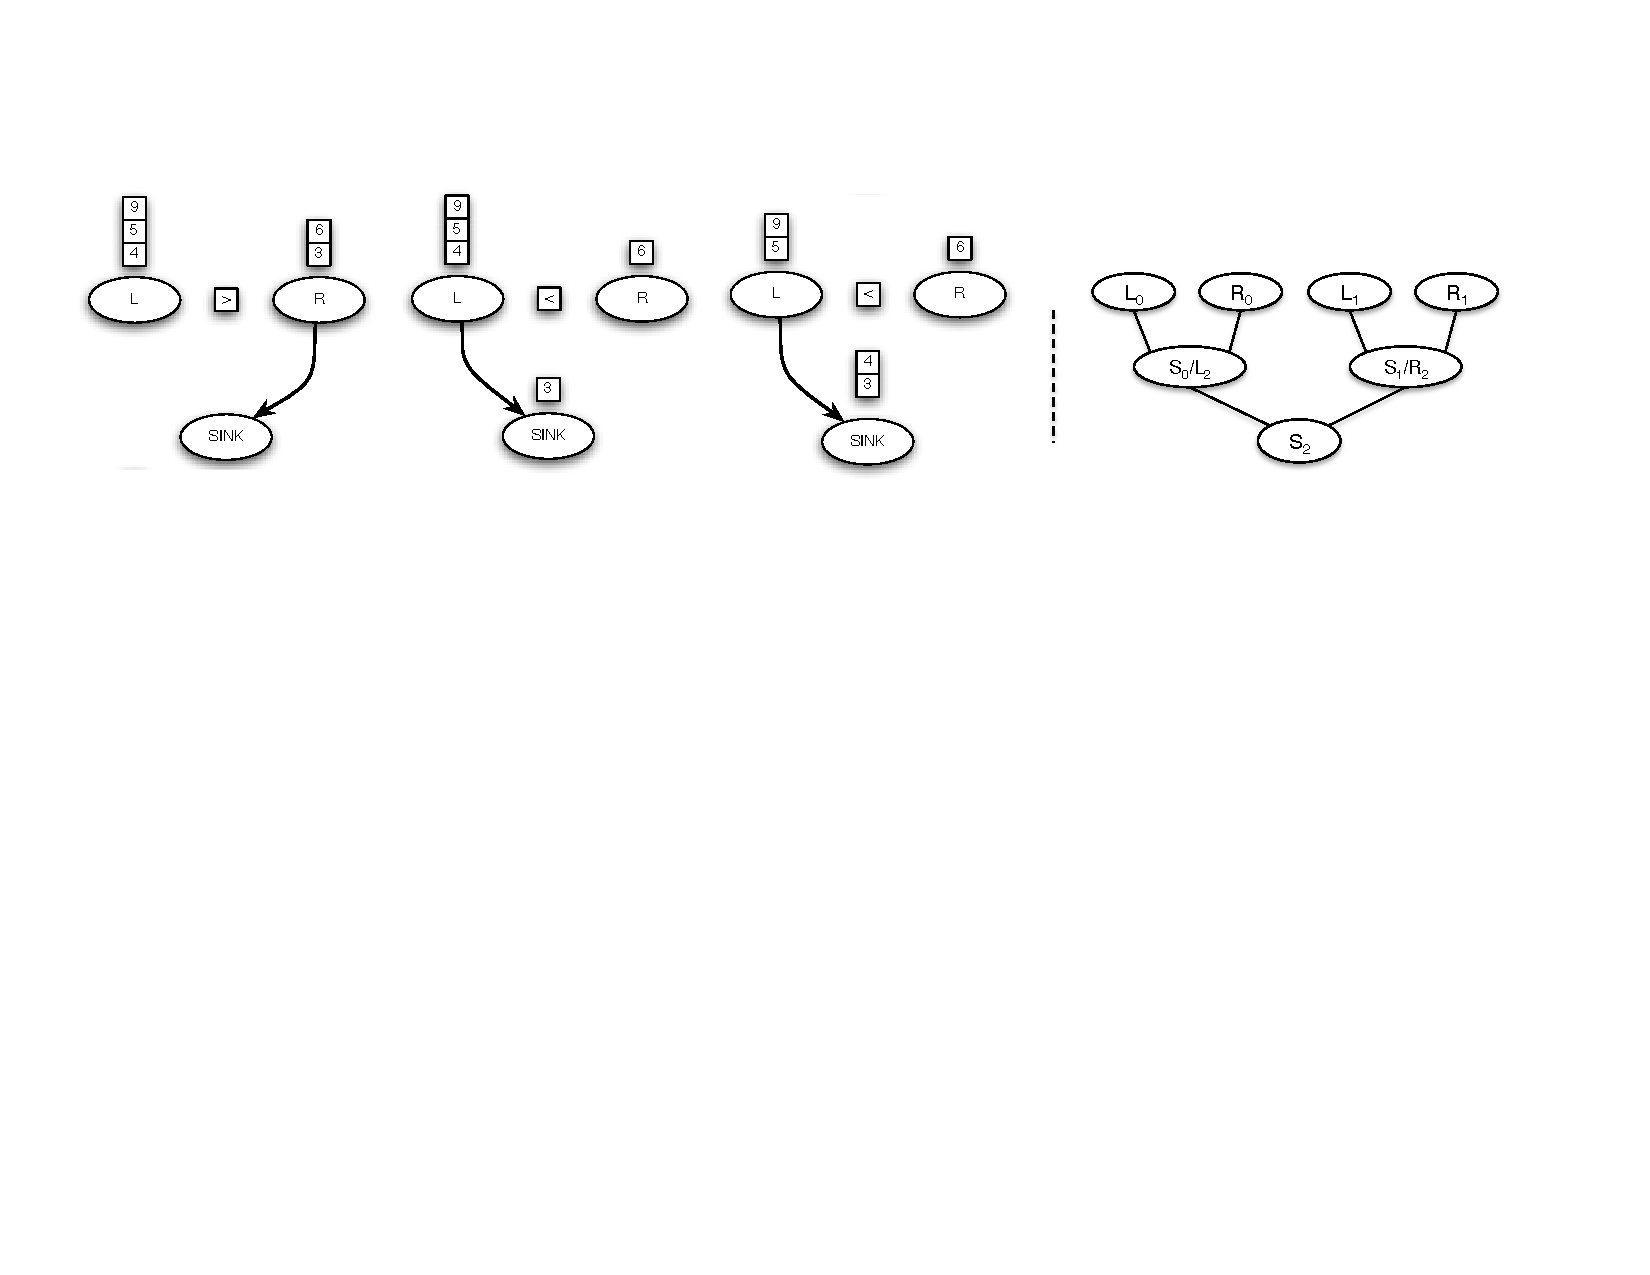
\includegraphics[width=0.95\textwidth]{graphics/online/pdaq/fig_hkn1_v2.pdf}
%  \caption{Left: the fundamental node of the Splicer, showing the
%    first few steps of merging / sorting two input streams.  Right: the
%    nodes connected into a tree, with inputs at the top and the output
%    stream at the bottom.  }
%  \label{fig:hkn1}
% \end{figure}

%The HKN1 (Hansen-Krasberg-1) algorithm at the core of the Splicer uses a tree
%of \emph{Nodes} to sort a constant number of time-ordered data streams.  Each
%Node contains a queue of pending data, a handle for a peer Node, and another
%handle for a sink Node (shared with the peer) to which sorted data is sent.

%The tree is assembled by associating each input stream with a separate Node
%and adding the Node to a list.  This list is then run through a loop which
%pulls off the first two Nodes, links them together as peers and creates a
%new Node which will act as the sink for both Nodes.  The new Node is then added
%to the list.  The loop exits when there is only one Node left.

%When a new piece of data arrives, it is added to the associated Node's queue.
%That Node then goes into a loop where it compares the top item from its queue
%with the top item from the peer's queue and the older of the two items
%is passed onto the sink Node (which adds the item to its queue and starts its
%own comparison loop.)  This loop stops as soon as the original Node or its
%peer has no more data.

%Generation of secondary streams.

%Along with physics data, DOMs produce three additional streams of data.
%The scaler data, monitoring the noise rate of each DOM in 1.6 ms bins,
%is used in the supernova data acquisition system \cite{IC3:supernova} to detect a
%global rise from many $O(10)$ MeV neutrino interactions occuring in the ice
%from a Galactic core-collapse supernova.  The time calibration and monitoring
%streams are used to monitor the health and quality of the data-taking runs.

As hits move from Omicron to the Sender, they are written to the
HitSpool, a disk-based cache of files containing hits.  These files are
written in a circular order so that the newest hits overwrite the oldest
data.  The first hit time for each file is stored in an SQLite database to
aid in fast retrieval of raw hit data.

One limitation of the current DAQ design is that it only reads data when
the DAQ is running, so the detector is essentially ``off'' during hardware
failures or the periodic full restarts of the system.  A future enhancement
will split the StringHub into several independent pieces to eliminate these
brief pauses.  The front end (Omicron) will be moved to an always-on daemon
that continuously writes data (including secondary, non-physics data and
other metadata) to the disk cache.  Part of the back end (Sender) piece
will become a simple HitSpool client which reads data from the disk cache
and sends it to the downstream consumers, while another simple component
will listen for time intervals from the Event Builder and return lists of
hits taken from the HitSpool.

\subsubsection{\label{sect:online:trigger}Triggers}

The DAQ trigger algorithms look for clusters of HLC hits in space and time
that could indicate light due to a particle interaction in the detector, as
opposed to uncorrelated dark noise.   An algorithm searches for a given
multiplicity of HLC hits, possibly with an additional geometric
requirement, within a trigger time window.  The time scale of the trigger window is
set by the light travel time in ice and the geometry requirement
involved. Longer readout windows are appended before and after the trigger
windows to save early and late hits with the events.

Triggers are generally restricted to a subset of DOMs, such as in-ice DOMs,
IceTop DOMs, or DeepCore DOMs.  The algorithms run in parallel over all
hits in the DOM set, and then overlapping triggers are merged.  The various
trigger algorithms are described below, and a summary of the algorithm
parameter settings is found in Table \ref{tab:triggers}.  Trigger settings
are changed at most once a year.

The fundamental trigger for IceCube, IceTop, and DeepCore is the Simple
Multiplicity Trigger (SMT).  The SMT requires $N$ or more HLC hits within a
sliding time window of several $\mu\mathrm{s}$, without any locality
conditions.  The trigger window is 
extended for as long as the multiplicity condition is satisfied.  The
multiplicity value $N$ is tuned to the energy threshold of the sub-detector,
which fundamentally is set by the string or tank spacing.

Other triggers use a lower multiplicity threshold by adding constrains on
the HLC hit topology.  The time windows for these triggers are based upon
the size of the locality volume. The Volume Trigger defines a cylinder of fixed size around
each hit DOM and requires a given multiplicity within this cylinder
(Fig.~\ref{fig:trig_cylinder}); this allows one to trigger on localized
low-energy events that do not satisfy the SMT condition.  The Volume Trigger
has an additional simple multiplicity parameter that fires the trigger when
reached, regardless of any spatial restrictions; this prevents the trigger
algorithm from slowing down when the detector has triggered already from
the primary SMT. The String Trigger requires a certain number of hits
within a span of DOMs along a single string 
(Fig.~\ref{fig:trig_string}); this allows one to trigger on low-energy
muons that pass vertically through the detector.

\begin{figure}[ht]
  \centering \subfloat[Schematic representation of the Volume Trigger.]{
    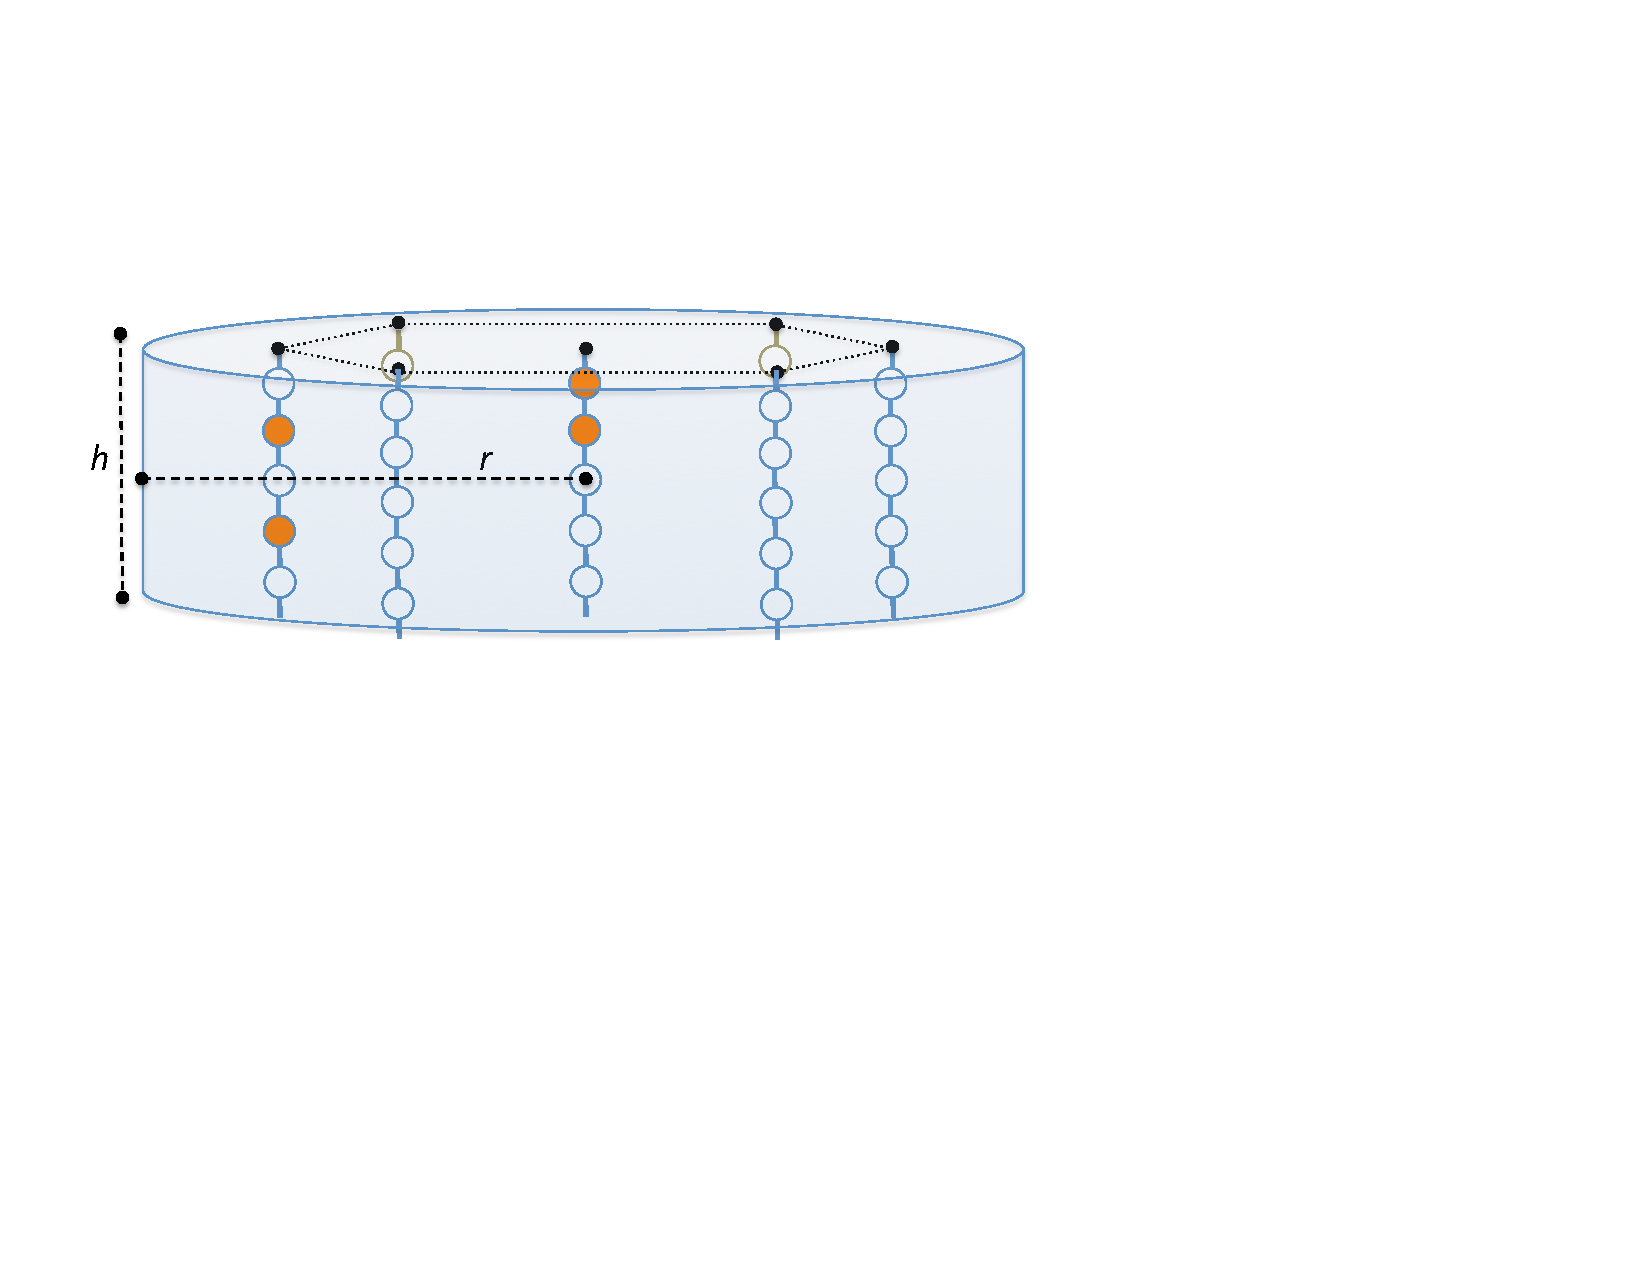
\includegraphics[scale=0.45]{graphics/online/trigger/trig_cylinder}
    \label{fig:trig_cylinder}
  } \quad \subfloat[Schematic representation of the String Trigger.]{
    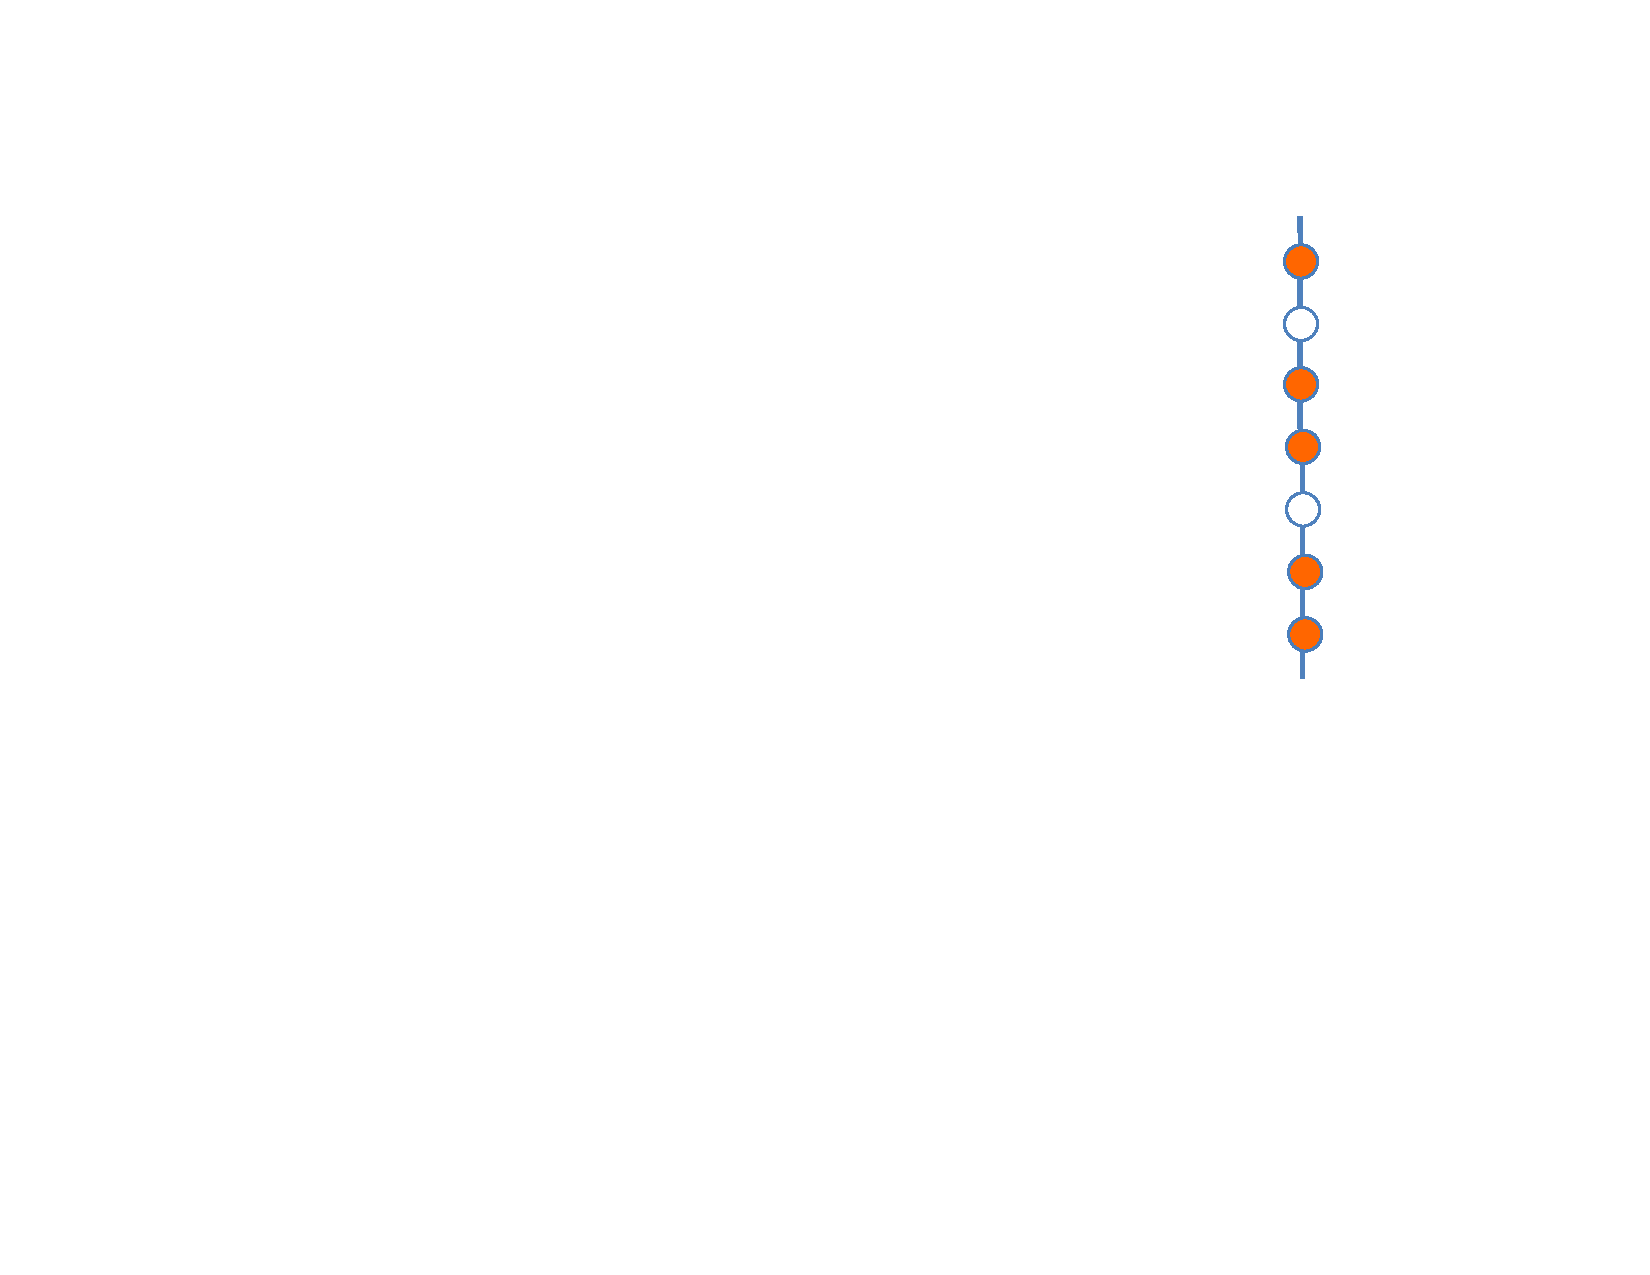
\includegraphics[scale=0.5]{graphics/online/trigger/trig_string}
    \label{fig:trig_string}
  }
  \caption{IceCube triggers using spatial coincidences.  Shaded circles
    represent HLC-hit DOMs.}
\end{figure}

IceCube has the potential to detect hypothetical subrelativistic heavy
particles such as magnetic monopoles, via catalyzed nucleon decays along
the particle trajectory \cite{IC3:monopole}.  However, because these
particles may travel at velocities $v \sim 0.001c - 0.01c$, the time
windows used in the standard triggers are too short.  A dedicated Slow
Particle (SLOP) trigger has thus been developed to search for slow
track-like particle signatures.

The SLOP trigger operates in several stages.  The HLC hits, which by design
come in at least pairs along a string, are cleaned by removing pairs that
are too close in time ($\Delta t < T_{\mathrm{prox}}$), removing many muon
hits.  Next, 3-tuples of HLC pairs within a time window $T_{\mathrm{max}}$
are formed.  The geometry of each 3-tuple formed must satisfy track-like
conditions: the obtuse inner angle of the triangle formed by the earliest
DOM in each pair must be larger than $\alpha_{\mathrm{min}}$, and the
``velocities'' along the triangle sides must be consistent.  Specifically,
the normalized velocity difference, defined as

\begin{equation}
  v_{\mathrm{rel}} = 3(v^{-1}_{12} - v^{-1}_{23})/(v^{-1}_{12} +
  v^{-1}_{23} + v^{-1}_{13})
\end{equation}

\noindent where $\ v_{ij} = \Delta x_{ij}/\Delta t_{ij}$, must be less than
or equal to a pre-definined maximum value
$v_{\mathrm{rel}}^{\mathrm{max}}$.  Fig.~\ref{fig:slop} shows the geometry
parameters of the 3-tuple.  Finally, the total number of track-like 3-tuples
must be greater than or equal to $N_{\mathrm{tuple}}$. 

\begin{figure}[!h]
 \centering
 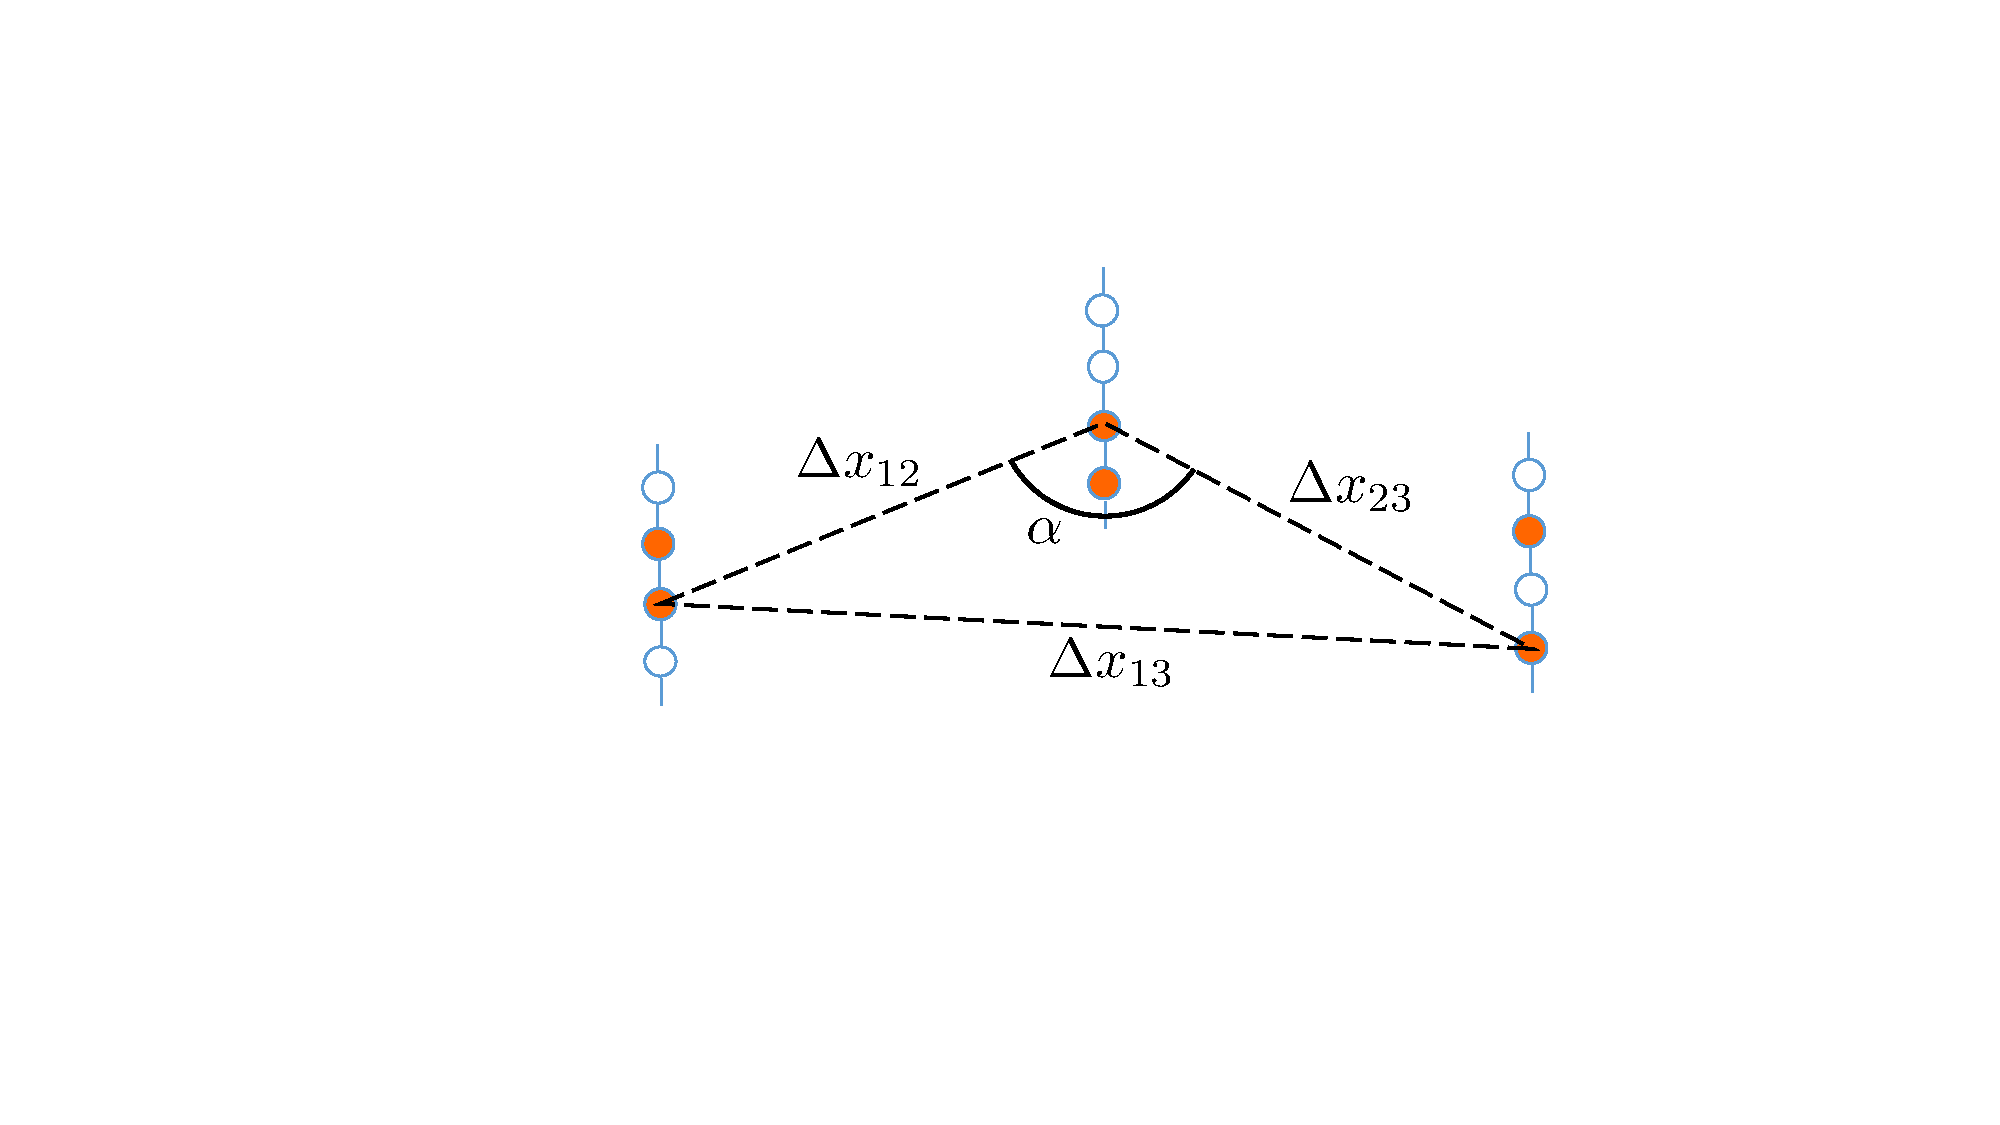
\includegraphics[width=0.8\textwidth]{graphics/online/trigger/slop.pdf}
 \caption{Geometry of a SLOP trigger HLC pair 3-tuple.}
 \label{fig:slop}
\end{figure}

Other special-purpose triggers exist to collect minimum bias data of
various sorts.  The Fixed-Rate Trigger (FRT) reads out 10~ms of data from
the full detector at fixed intervals.  This is especially useful for studies
of DOM noise.  The Calibration Trigger selects a particular type of hit
such as special IceTop non-LC hits that have full waveform readout, and promotes
them to a trigger. The Calibration Trigger can also be configured to
include all events due to LED flashers in cases where flasher 
operations require disabling standard triggers. Finally, a Minimum Bias
trigger can select $1/N$ HLC hits and promote the hit to a trigger, adding
readout windows as usual; currently an IceTop Minimum Bias trigger with a
prescale factor of 10000 is active.

\begin{table}
  \centering \footnotesize
\begin{tabular}{lrrrrr}
  \hline Trigger & DOM set & $N$ HLC hits & Window & Topology & Rate\\ & &
  & ($\mu$s) & & (Hz) \\ \hline SMT & in-ice & 8 & 5 & --- & 2100\\ SMT &
  DeepCore & 3 & 2.5 & --- & 250\\ SMT & IceTop & 6 & 5 & --- & 25\\ Volume
  & in-ice & 4 & 1 & cylinder (r=175m, h=75m) & 3700\\ Volume & IceTop core
  & 4 & 0.2 & cylinder (r=60m, h=10m) & 4\\ String & in-ice & 5 & 1.5 & 7
  adjacent vertical DOMs & 2200\\ SLOP & in-ice & $N_{\mathrm{tuple}} = 5$
  & $T_{\mathrm{prox}} = 2.5$ & $\alpha_{\mathrm{min}} =
  140^\circ,\ v_{\mathrm{rel}}^{\mathrm{max}} = 0.5$ & 12\\ & & &
  $T_{\mathrm{max}} = 500$ & $\alpha_{\mathrm{min}} =
  140^\circ,\ v_{\mathrm{rel}}^{\mathrm{max}} = 0.5$ & 12\\ FRT & all & ---
  & --- & --- & 0.003\\ \hline
\end{tabular}
\caption{IceCube trigger parameters (as of May 2016) and typical trigger
  rates of each algorithm.  Most rates vary seasonally with the atmospheric
  muon flux.}
\label{tab:triggers}
\end{table}

Many events will satisfy more than one of the trigger conditions, sometimes
multiple times.  In order to avoid overlapping events, possibly containing
the same DOM hits, the triggers and their associated readout windows are
merged, while retaining information about the separate triggers.  The
merged trigger is referred to as the Global Trigger.

Each trigger has defined readout windows around the trigger window; all
hits from the full detector, those DOM sets not involved in the trigger,
are requested from the StringHub components and built into events.  For the
DOM set involved in the trigger, the readout windows are appended at the end of the trigger
window, while for other DOM sets, the readout windows are centered around
the trigger start time.  The union of overlapping readout windows defines
an event (Fig.~\ref{fig:trigger_readout}).  Long events such as SLOP or FRT
triggers typically contain several causally independent ``physics'' events;
these typically are re-split before reconstruction and analysis.

\begin{figure}[!h]
 \centering
 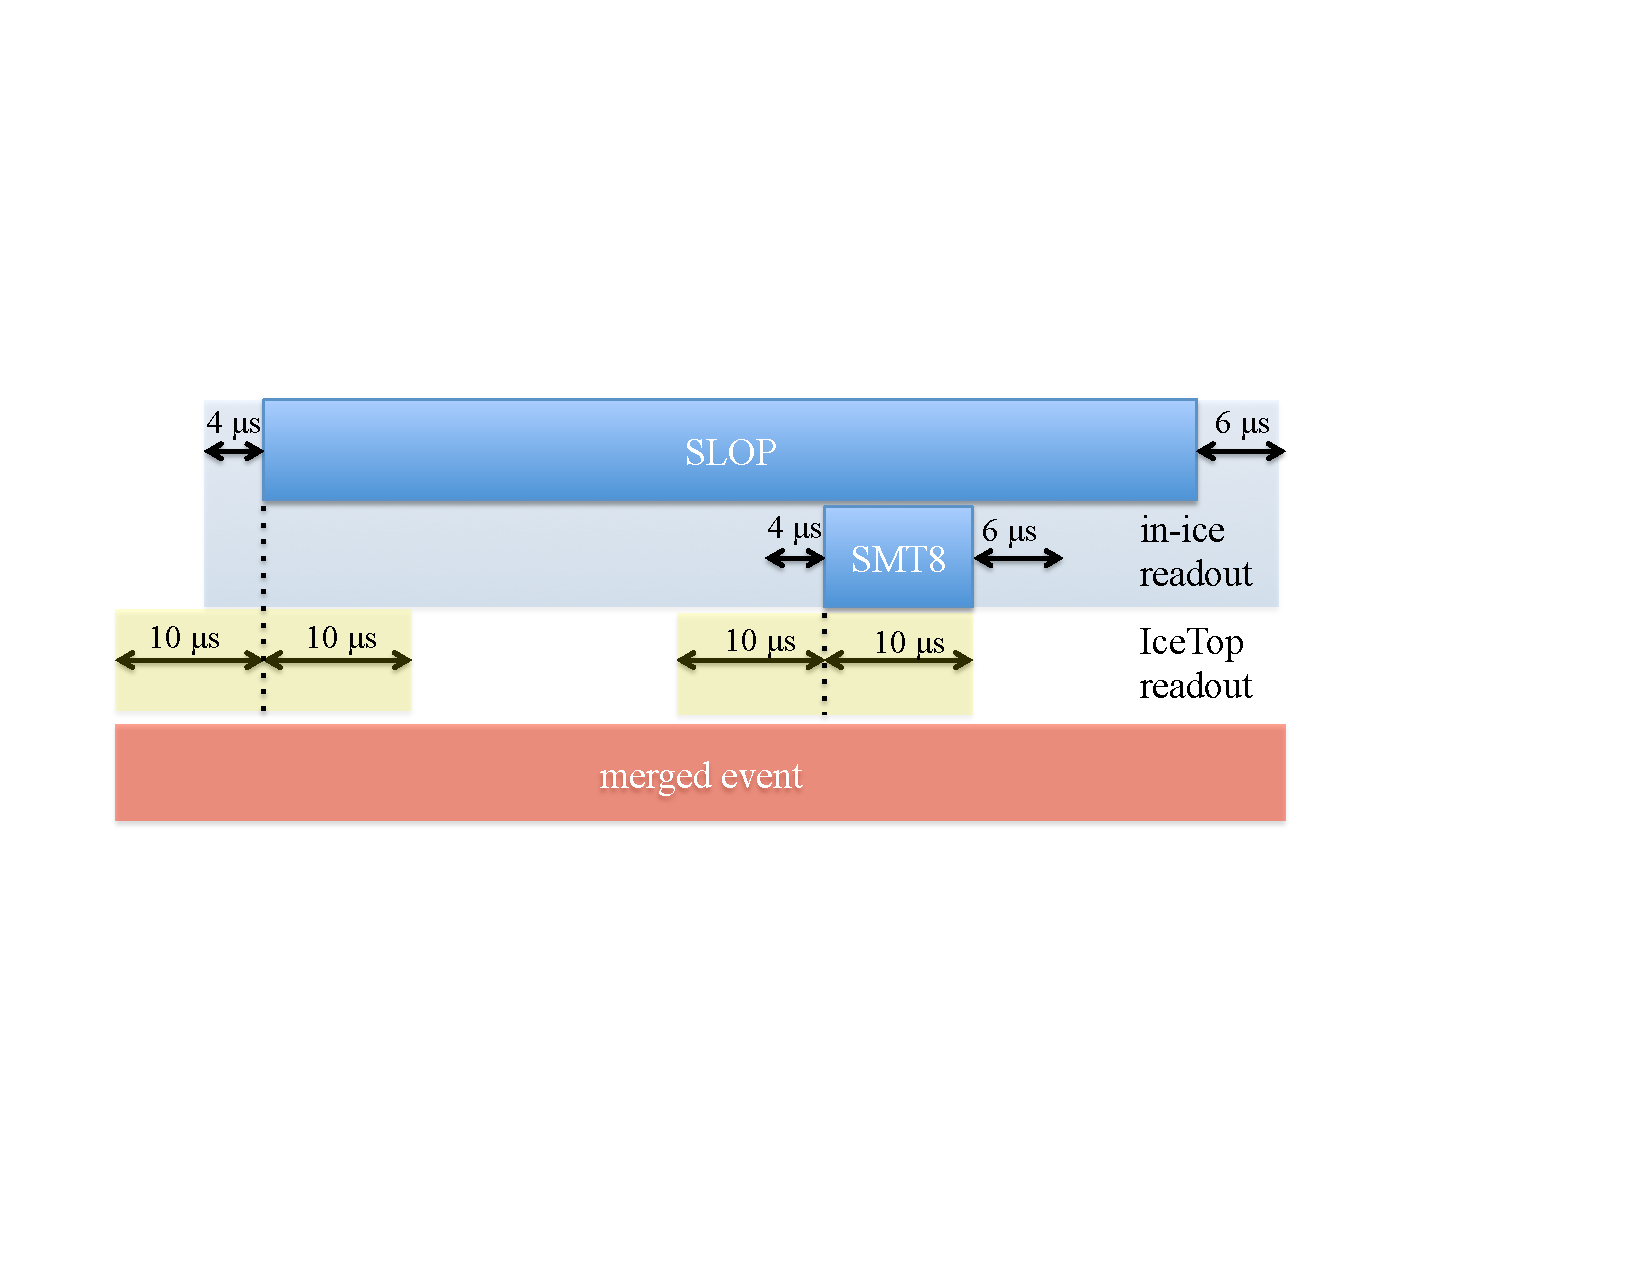
\includegraphics[width=0.8\textwidth]{graphics/online/trigger/trigger_readout}
 \caption{In-ice, IceTop, and merged readout windows for a long event
   satisfying SLOP and SMT8 triggers (not to scale).}
 \label{fig:trigger_readout}
\end{figure}

% \begin{figure}[ht]
%   \centering
%   \subfloat[Sample bright event satisfying multiple triggers.  The vertical ticks
%     indicate the time of DOM hits (including SLC hits).  Trigger windows are
%     illustrated with solid horizontal lines, readout windows by dashed lines.]{
%     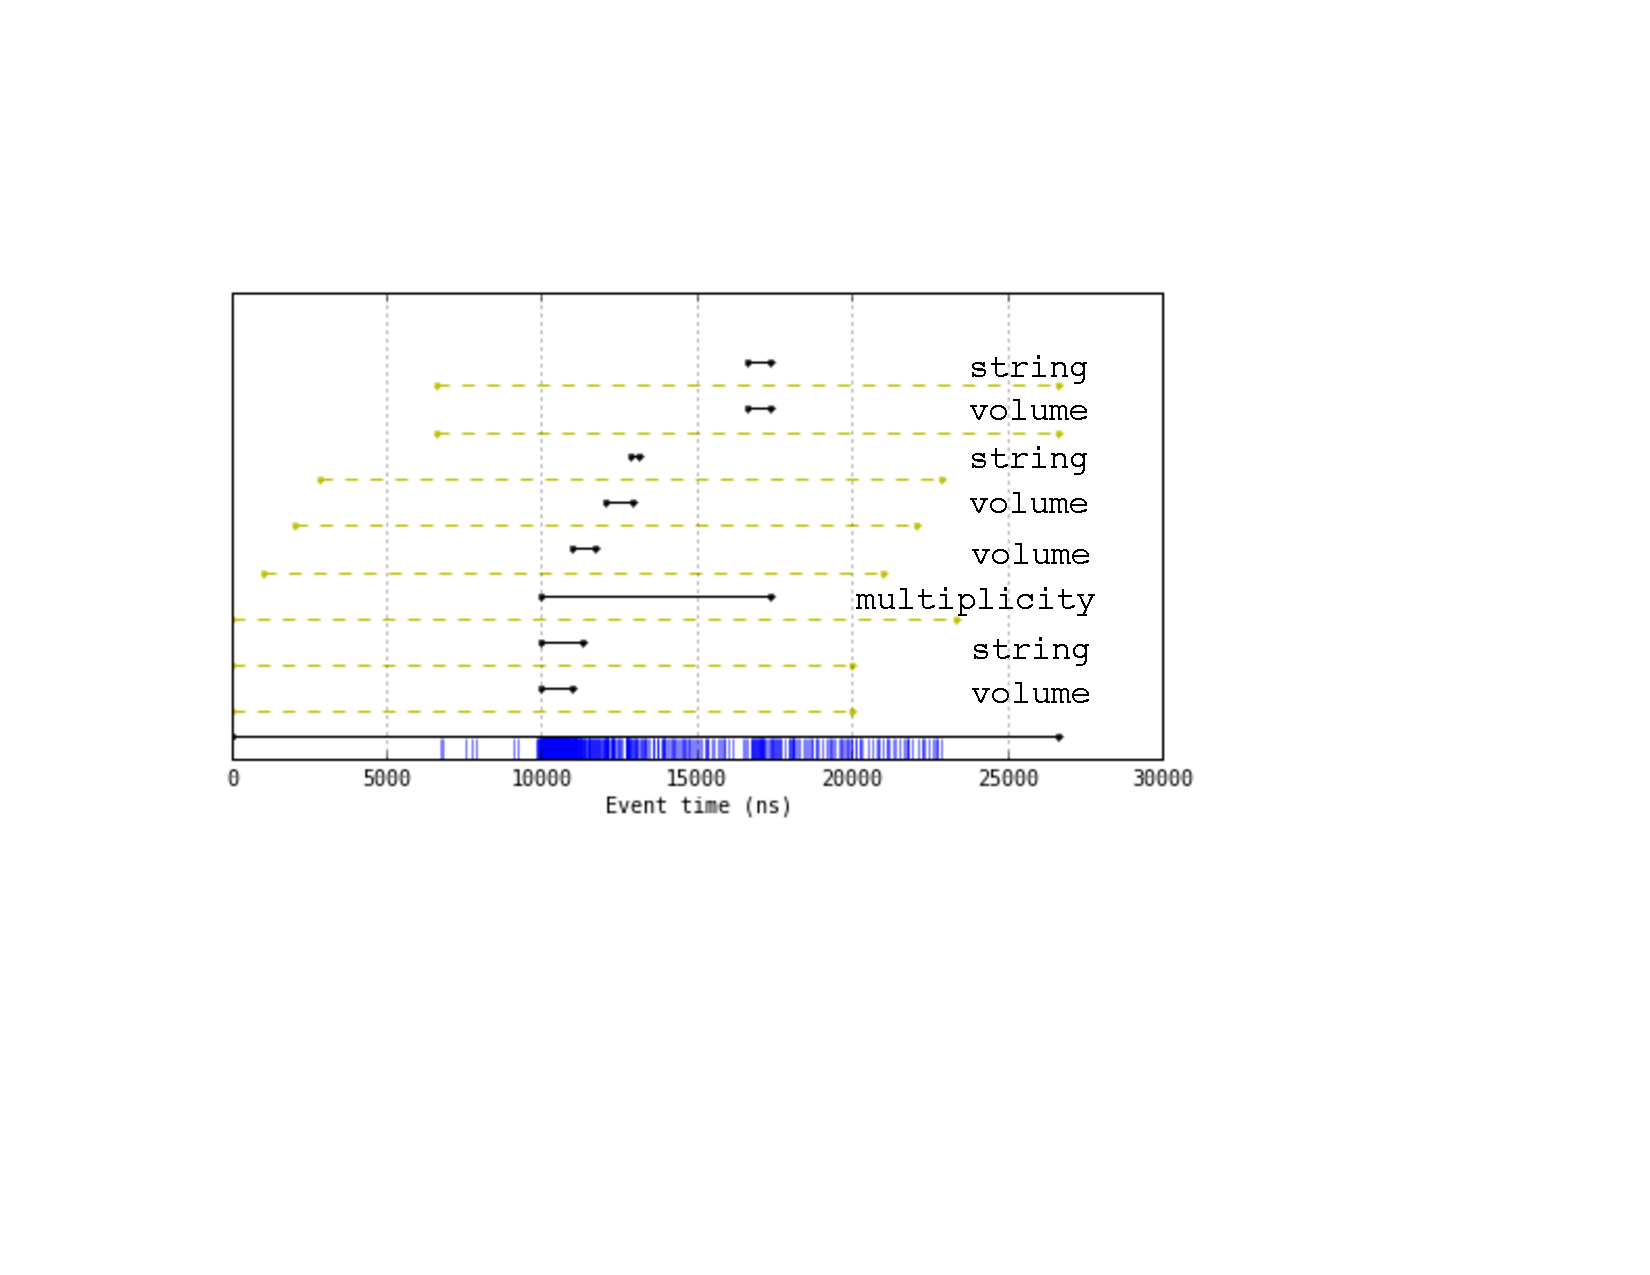
\includegraphics[scale=0.5]{graphics/online/trigger/trigger_example}
%     \label{fig:trigger_example}
%   }
%   \quad
%   \subfloat[In-ice, IceTop, and merged readout windows for a long event
%     satisfying SLOP and SMT8 triggers (not to scale).]{
%     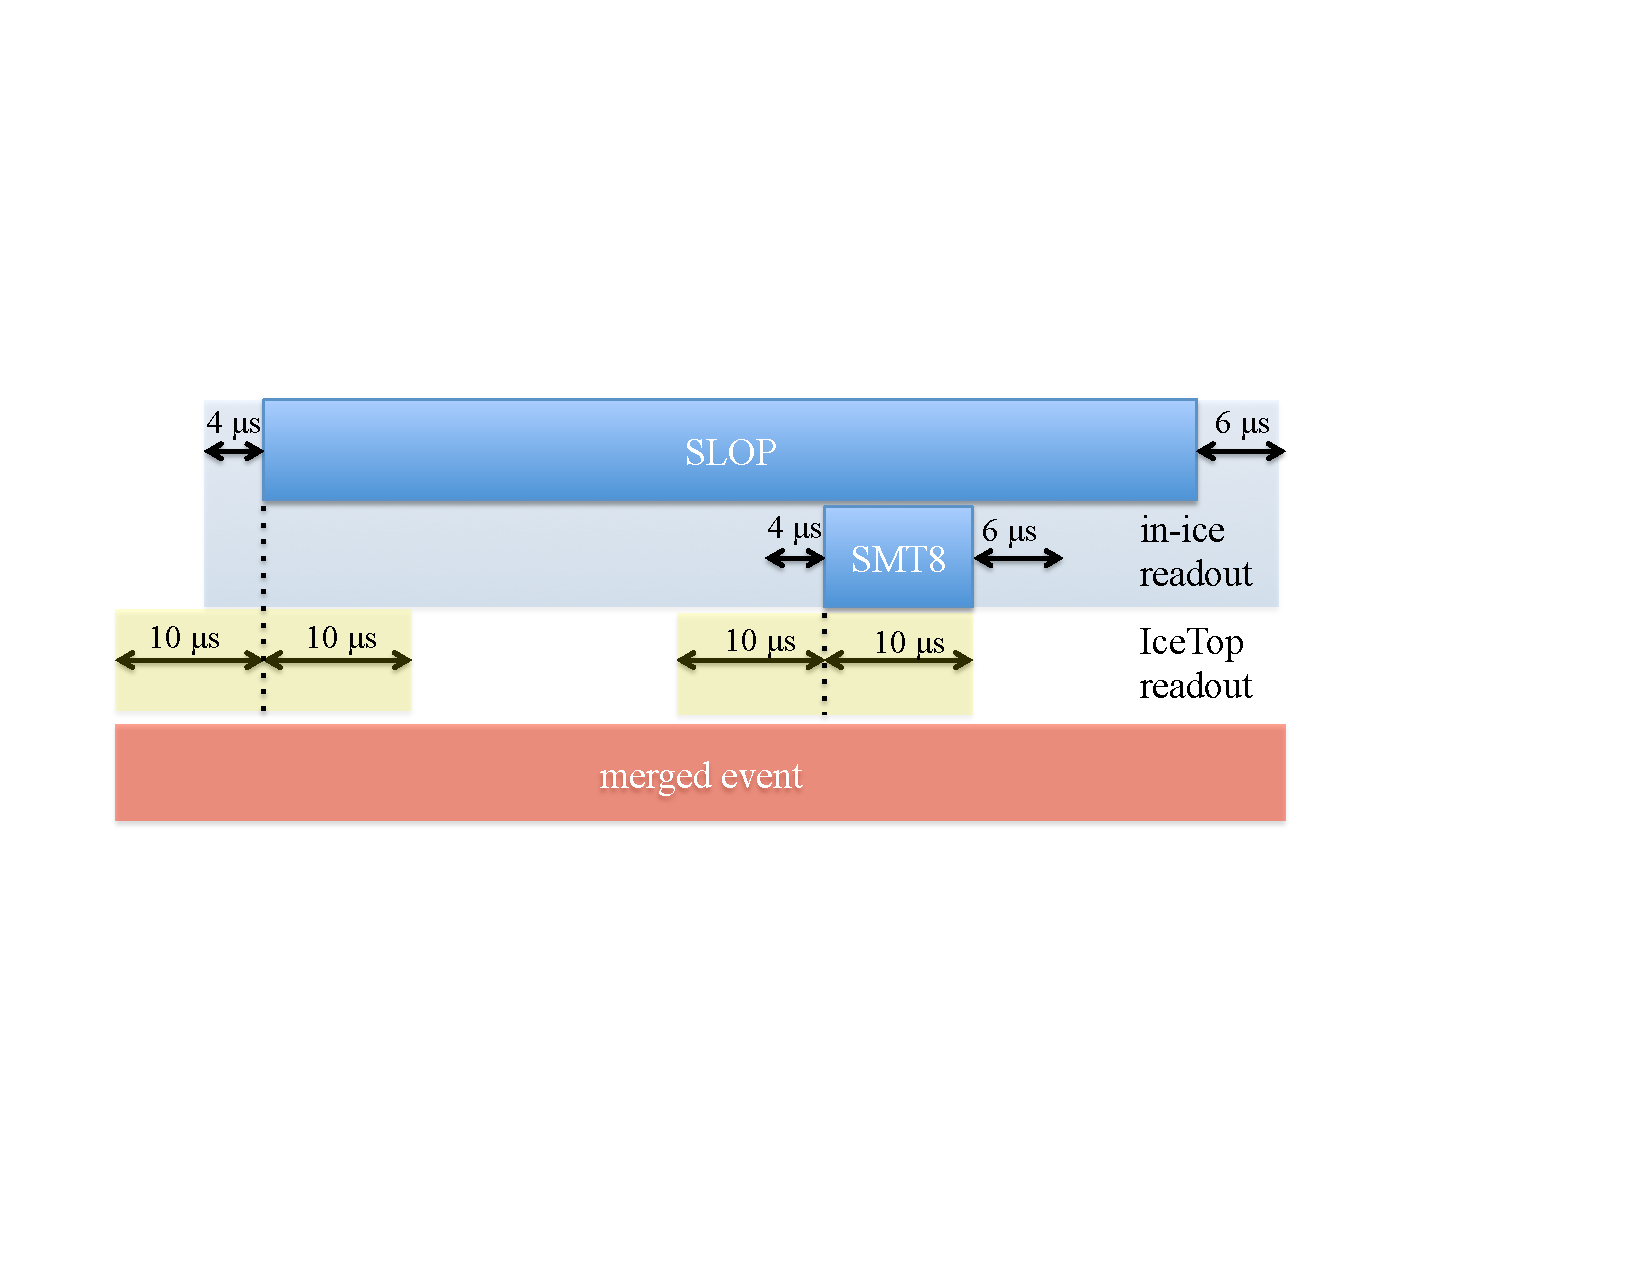
\includegraphics[scale=0.5]{graphics/online/trigger/trigger_readout}
%     \label{fig:trigger_readout}
%   }
%   \caption{IceCube trigger and readout window merging.}
% \end{figure}

\subsubsection{\label{sect:online:evbuilder}Event Building}

The Event Builder receives requests from the Global Trigger, extracts the
individual readout windows, and sends them to the appropriate subset of the
StringHubs.  The StringHubs each send back a list of all hits within the
window.  When all StringHubs have returned a list of hits, extraneous data is
removed from the trigger, and hit payloads and bundled into an event payload.

Events are written to a temporary file.  When the temporary file reaches a
configurable size, it is renamed to a standard unique name.  When the PnF
system sees a new file, it accepts it for processing and filtering.

\subsubsection{DAQ and DOM Configuration}

Configuration of the DAQ is managed by two sets of XML files; a cluster
configuration file and a hierarchical tree of run configuration files.

The cluster configuration file contains system-level settings used to
launch the DAQ, such as component host servers, startup paths, command-line
options, etc.  Components (other than StringHub) can easily be moved to
different hosts for troubleshooting, load balancing, and maintenance.

Run configuration files list the trigger and DOM configuration files to be
used for taking data.  The trigger configuration file specifies
configuration parameters for all 
trigger components (in-ice, IceTop, and global) used in a run.  These
include the list of algorithms run by each trigger component, along with
readout window sizes and any other configurable parameters (frequency,
threshold, etc.).

DOM configuration files (one per hub) list all DOMs that contribute to
the data-taking run.  All configuration parameters for each DOM are
specified, including PMT high voltages, ATWD operating parameters,
discriminator thresholds, local coincidence settings, and others.

Run configuration files (including trigger and DOM files) are versioned and
frozen once used for data-taking.  All relevant configuration parameters
are also stored in a database for use in analysis.

\subsubsection{Component Control}

The DAQ components are managed by a single ``command-and-control'' daemon,
CnCServer, that manages and monitors components, and acts as the main
external interface to the DAQ.  It uses a standard component interface to query and
control the components, and a separate interface for components to expose
internal data used for monitoring the health of the detector or for
debugging purposes.

CnCServer dynamically discoveres the detector components during a launch
phase, and instructs them to connect as needed.  Using the run
configuration files, it then distributes each component configuration
appropriately.  The components are then started to begin a data-taking run.
When a run is in progress, CnCServer regularly checks that components are
still active and that data is flowing between components.

%CnCServer starts out knowing nothing about the detector components.  During the
%DAQ's launch phase, components are given the host and port used by CnCServer.
%When components start up, each one sends CnCServer its name, host/port pairs,
%and the types of inputs and outputs it expects, and CnCServer adds them to its
%internal list.

%To start a run, CnCServer is given the name of the run configuration.  That
%run configuration may include all components or only a subset.  Using
%that file, CnCServer builds a list of components required for the run.
%Each of the included components is told to connect to their downstream
%neighbor, then to use the run configuration to initialize as appropriate
%(configure DOM hardware, initialize trigger algorithms, etc.).
%Once all components are successfully
%configured CnCServer instructs them to start, working its way from the Event
%Builder back to the String Hubs.

%When a run is in progress, CnCServer regularly checks that components are still
%active and that data is flowing between components.  If it detects a problem,
%it stops the run and relaunches all the components.  CnCServer also
%periodically collects all components' monitoring data and writes it to
%monitoring files which can be used for post-mortem diagnosis of detector
%failures.

\subsubsection{\label{sect:SNDAQ}Supernova Data Acquisition System}

The IceCube DAQ has a parallel triggering and analysis pathway designed
specifically for the detection of the many $O(10)$ MeV neutrinos from a
Galactic core-collapse supernova.  In the case of such an event, these
neutrinos will produce interactions in
the detector that, individually, are too dim to trigger the standard DAQ,
but because of their high multiplicity, can cause a coherent rise in the
individual hit rate of all of the in-ice DOMs~\cite{IC3:supernova}.

Each DOM monitors its hit rate and sends a stream of binned counts, using a
bin width of 1.6384~ms ($2^{16}$ 40MHz clock cycles).  An artificial
deadtime of $250\ {\mu}\mathrm{s}$ is applied after each trigger to reduce the
impact of correlated afterpulses (see Sec.~\ref{sect:darknoise}).  Each
StringHub collects the rate stream of each DOM, supplies UTC timestamps,
and forwards the streams to the Secondary Builder.

The supernova DAQ (SNDAQ) system receives the Secondary Builder stream,
rebins the individual DOM rates, and monitors the sum of rates for a
significant rise over several timescales.  This analysis is described in
detail in Ref.~\cite{IC3:supernova}.  One complication is that short-term
fluctuations in the cosmic ray muon rate can affect the significance
calculation.  To correct for this, the trigger rate of the standard DAQ is
continuously sent to SNDAQ, and any significant alert is corrected
\cite{IC3:icrc15_sndaq}.  At a high significance threshold, the capture of
all untriggered data around the alert time is initiated using the HitSpool
system (Sec.~\ref{sect:hitspool}), and the Supernova Neutrino Early Warning
System (SNEWS) \cite{SNEWS} is notified.

\subsubsection{\label{sect:hitspool}HitSpool Request System}

Subsystems such as SNDAQ can send time interval requests to a HitSpool
Request daemon to collect raw data from significant transient events. At
the time of this writing, the HitSpool Request System has three clients;
their basic characteristics are described in
Table~\ref{tab:hsclients}.  The central daemon passes the request onto 
every DOMHub, where ``worker'' daemons gather the hits in the requested time
interval and forward them a single ``sender'' daemon
that bundles them up to be transferred to the Northern Hemisphere for further analysis.

SNDAQ requests HitSpool data from an asymmetrical time window of $90
\,\mathrm{s}$ around a supernova alert with a significance $\xi > 7.65$,
and data from a symmetrical $500\,\mathrm{s}$ window around a trigger with
significance $\xi > 10.0$.  The online High Energy Starting Event (HESE)
analysis system requests HitSpool data from a symmetrical time window of
1~s around events with a total deposited charge of greater than 1500~PE.
The recently implemented HitSpool client for solar flare analyses is
triggered externally by significant FERMI-LAT events and requests HitSpool
data from a symmetrical time window of one hour around the trigger
time. Unlike the other two clients, these data sets are not transferred
over the satellite due to their size but are stored locally on disk, with
transmission over satellite only allowed in extraordinary cases.

\begin{table}
  \caption{HitSpool data-requesting services and request characteristics.}
  \centering
  \footnotesize
\begin{tabularx}{\textwidth}{XXXXXXX}
  \toprule Client & Trigger Threshold & Time Window & Request Length & Raw
  Data Size & Frequency & Bandwidth \\
  \midrule SNDAQ & $7.65 \,\xi$
  ($10.00 \,\xi$) & $[-30\,\mathrm{s},+60\,\mathrm{s}]$ ($[\pm250
    \,\mathrm{s}]$)& $90 \,\mathrm{s}$& ~ $18 \,\mathrm{GB}$&
  $0.5/\mathrm{week}$ ($0.0006 / \mathrm{week}$)& $1.3 \,\mathrm{GB} /
  \mathrm{day}$\\ HESE & $1500 \,\mathrm{PE} $ ($6000 \,\mathrm{PE} $) &
  $[\pm0.5\,\mathrm{s}]$& $1\,\mathrm{s}$ & $~150\,\mathrm{MB}$ &
  $4/\mathrm{day}$ ($1/\,\mathrm{month}$) & $0.4\,\mathrm{GB}/\mathrm{day}$
  \\
  Solar Flare & FERMI-LAT & $[\pm30\,\mathrm{min}]$ & $1\,\mathrm{h}$&
  $~600\,\mathrm{GB}$& $ 7 / \mathrm{year}$& $ 1.7
  \,\mathrm{GB}/\mathrm{day}$\\ & significant event & & & & &
  \\ \bottomrule
\end{tabularx}
\label{tab:hsclients}
\end{table}

\subsection{\label{sect:online:filter}Online Processing and Filtering}

\subsubsection{Overview}

The online Processing and Filtering (PnF) system is charged with the immediate
handling of all triggered events collected by the DAQ
and reducing the data volume to a level that can be accommodated in our
satellite bandwidth allocations ($\sim$100 GB/day).  This treatment
includes application of calibration constants, application of event
characterization and selections, extracting data quality monitoring
information, generation of realtime alerts for events of astrophysical
interest, and creation of data files and metadata information for long-term
archiving.  The PnF system is a custom software
suite that utilizes $\sim$20 standard, multi-processor servers located in
the SPS computing cluster.  

Each triggered event consists of a collection of digitized
waveforms recorded by the DOMs~\cite{ref:domdaq}.  To be
useful for physics, each of these waveforms requires application of
calibration constants that allow the waveform units to be converted from
the raw units (ADC counts per sample bin) to more physical units (mV
measured in each fixed time, 3.3 ns bin).  These calibration constants are
independently measured (see Sec.~\ref{sec:domcal}) and stored in an online
database for use by PnF.  Next, each
DOM's waveform is deconvolved using the known DOM response to photons to
extract the light arrival time and amplitude information~\cite{IC3:ereco}.
This series of time and amplitude light arrival information for each DOM is
the base for event reconstruction and characterization.  PnF encodes this
information in a compact data format known as the Super Data
Storage and Transfer format (SuperDST), and occupies 9\% of the storage
size of the full waveform information.  The encoding does introduce a
small level of discretization error to the data, measured to be 1.1~ns in time and
0.04~PE in charge, and smaller than the calibration uncertainties on these
values.  Any DOM readout whose SuperDST information is found not to be a
good representation of the original waveform, or sees very high amounts of
light, also has the full waveform readout saved in addition to the
SuperDST record.

% JVS internal study on discretization:  
% https://events.icecube.wisc.edu/getFile.py/access?contribId=140&sessionId=4&resId=0&materialId=slides&confId=33

Each event is then characterized with a series of reconstruction
algorithms that attempt to match the observed patterns of recorded light in
the SuperDST with known patterns of light from track and showering event
hypotheses~\cite{IC3:ereco}.  The reconstructed location, direction,
energy, and the goodness-of-fit are used to select interesting events by various
filter selections.  The filter criteria are set by the collaboration
each year and are tuned to select events of interest to specific
analyses.  Each year there are about two dozen unique filter selections in
operation.  Some of these filters are designed to search for
neutrino events of wide astrophysical interest to the scientific community
and trigger alerts that are distributed to followup observatories
worldwide~\cite{Abbasi:2011ja,Aartsen:2015trq}.

The PnF system also extracts and aggregates data quality and monitoring
information from the data as is it processed.  This information includes
stability and quality information from the DOM waveform and calibration
process, rates of DOM readouts, and rates and 
stability information for all detector triggers and filters.  This
information is aggregated for each data segment and reported to the IceCube
Live monitoring system (Sec.~\ref{sec:online:icecubelive}).

Finally, the PnF system generates several types of files for satellite
transmission and as the long-term data archive of the experiment. These
include:   
\begin{enumerate}
\item Filtered data files containing only events selected by the online filter
  selections.  These events generally only include the SuperDST version of
  the DOM information and results from the online event reconstructions.
  These files are queued for satellite transmission to the IceCube data
  warehouse by the data handling system.
\item SuperDST data files containing the SuperDST version of DOM readout
  information for all triggered events as well as summary information from
  the online filtering process.  This file set is intended as the long-term
  archive version of IceCube data.
\item Raw data files containing all uncalibrated waveforms from all DOMs for
  every event.  This large data set is saved until final data quality
  assurance on the SuperDST sample can be completed.
\end{enumerate}

During normal operations, the DAQ produces a raw data output of $\sim$1 TB
of raw data per day, which results in a raw data file 
archive of the same size.  The SuperDST and filtered data archive, after
data compression, are $\sim$170 GB/day and $\sim$90 GB/day, respectively.

\subsubsection{System Design}

The online processing and filtering system uses a modular design, where
each component is responsible for a portion of data processing built around
a central master server node and a scalable number of processing client
nodes.  The central master server focuses on data distribution and
aggregation tasks (requesting data blocks from the DAQ, collating event
SuperDST, reconstruction, filter, and monitoring information and writing
data files), while the client process focus on the per-event processing
tasks (event calibration, reconstruction, analysis, and filtering).

The system is built upon the IceCube analysis software framework,
IceTray~\cite{DeYoung:2005zz}, allowing standard IceCube algorithms to be
used in the online processing and filtering system without modifications.
Additionally, the system uses the Common Object Request Broker Architecture
(CORBA) system as means for controlling, supervising and interconnecting
the modular portions of the system.  Specialized classes are used to
provide CORBA interconnections within the IceTray system, allowing
file-like interfaces that let data to stream from one component to another
using native IceTray formats.  Use of a CORBA name server and a dynamic
architecture allow for the addition and remove of filtering clients as
needed to meet the processing load from annual filtering changes and
overall rate variations from seasonal variations in the detector trigger
rate or moving system components within the SPS computer system as needed.

\subsubsection{Components}

The flow of triggered event data in the online processing and filtering
system is shown in Fig.~\ref{fig:online_pnf_internals} highlighting the
flow of data from the DAQ system, though the master server and clients, to
files on disk and online alerts.  Several standard components include:
\begin{enumerate}
\item DAQ Dispatch is a process to pickup event data from the data
  acquisition system data cache and forward to the PFServer components.
\item Central Servers are central data flow managers within the online
  processing and filtering system.  These servers receive data from the
  I3DAQDispatch event source, distribute events to and record results
  returning from the PFClient farm, and send events to file, monitoring and
  alert writing components.  Typically there are 4 servers used in
  operation.
\item Filter Clients are where the core calibration, reconstruction and
  filtering processs are applied to each triggered event.  In normal
  operation, up to 500 of these clients operate in parallel to filter
  events in real time.
\item GCD Dispatch is a database caching system to prevent the ~400
  PFClient processes from overwhelming the database system when requesting
  geometry, calibration and detector status (CGD) information.  This system
  aggregates database requests, makes a single database query and shares
  the results with all PFClients.
\item File Writers are responsible for creation of files and meta-data for
  the IceCube data archive.  These files are written in standard IceTray
  file format.  There is one writer component for each file type created.
\item Online Writer is responsible for extracting event reconstruction and
  filter information from the data for events of astrophysical interest and
  sending this information out in real time via the IceCube Live alert
  system.
\item Monitoring Writer is responsible for aggregating per-event monitoring
  information, creating histograms and forwarding them to the IceCube Live
  monitoring system.
\item Filtered Data Dispatch and FollowUp clients are responsible for
  looking for bursts of neutrino events on timescales from 100 seconds up
  to 3 weeks in duration. This post-filtering search of the data has all
  filter-selected events available, enabling event to event correlations to
  discovered.  Any significant burst of neutrinos found generates alerts
  sent to partner observatories worldwide.
\end{enumerate}

\begin{figure}[!h]
 \centering
 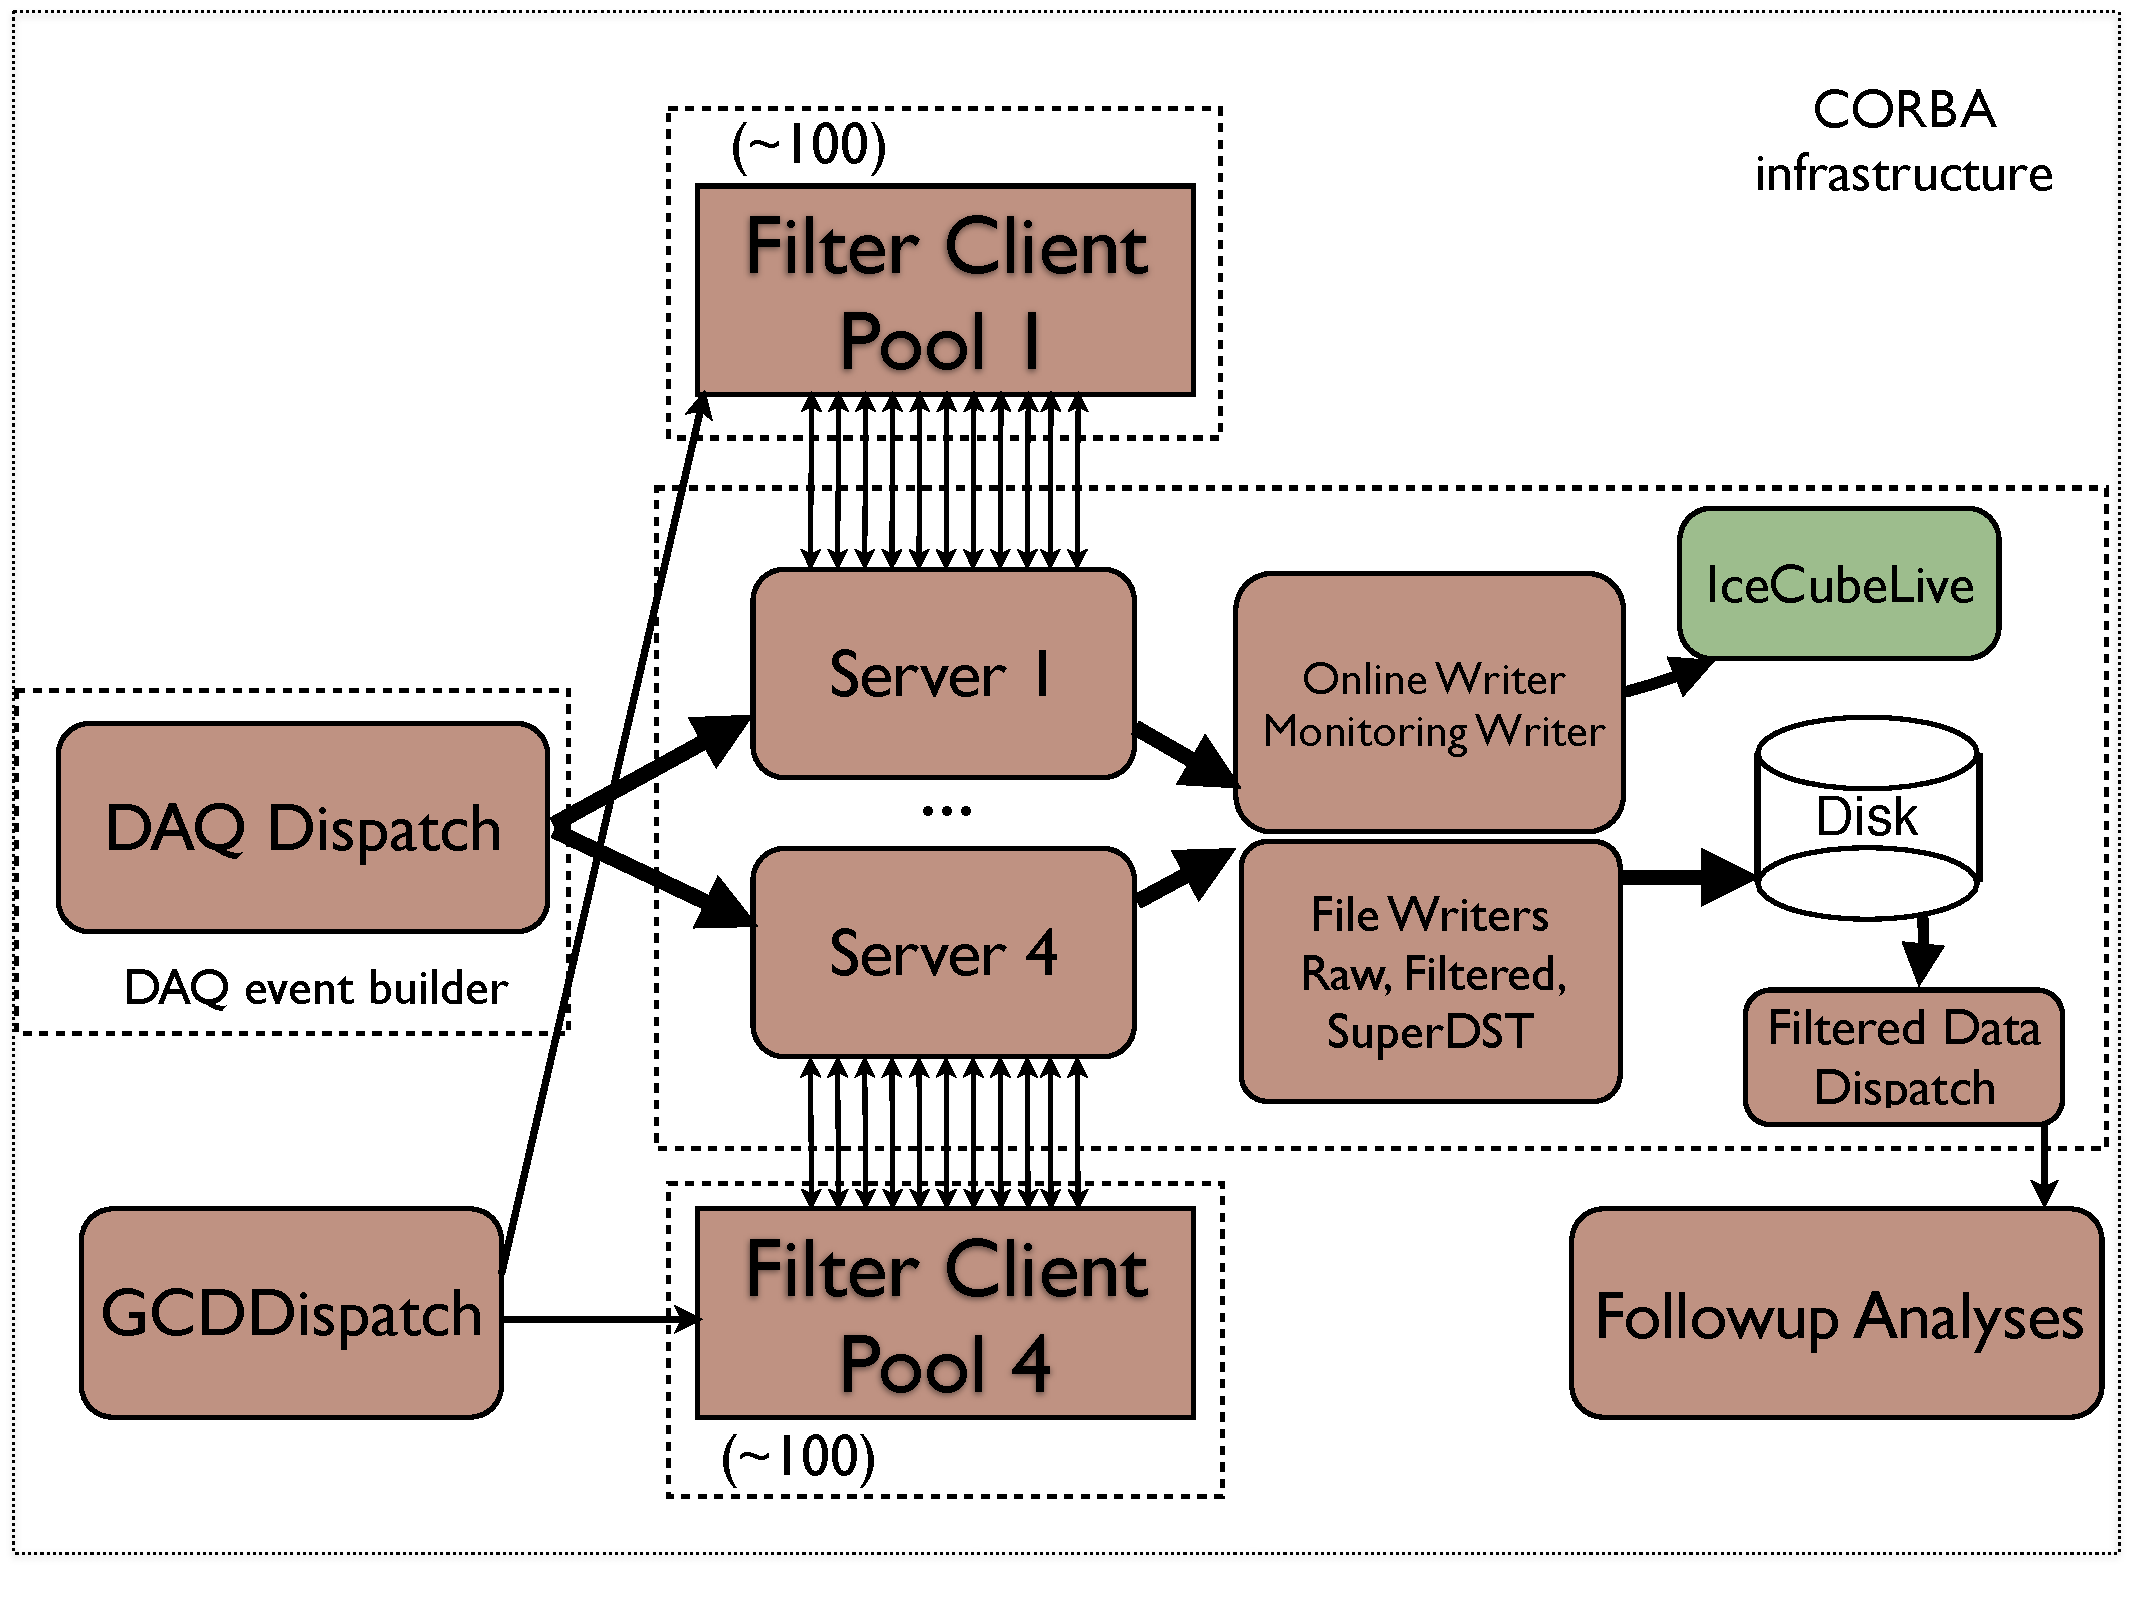
\includegraphics[width=0.8\textwidth]{graphics/online/pnf/PnF_Internals.pdf}
 \caption{Internal components of the Online Processing and Filtering
   System.  Arrows highlight the flow of data within the system.}
 \label{fig:online_pnf_internals}
\end{figure}

\subsubsection{Performance}
The online processing and filtering system is designed to filter triggered
events as quickly as possible after collection by the data acquisition
system.  A key metric is processing system latency, defined as the duration
of time between the data acquisition trigger and the completion of event
processing and filtering.  A typical latency history for the system is
shown in Fig.~\ref{fig:online_pnf_latency}, showing typical system
latencies of $\sim$20 seconds.

\begin{figure}[!h]
 \centering
 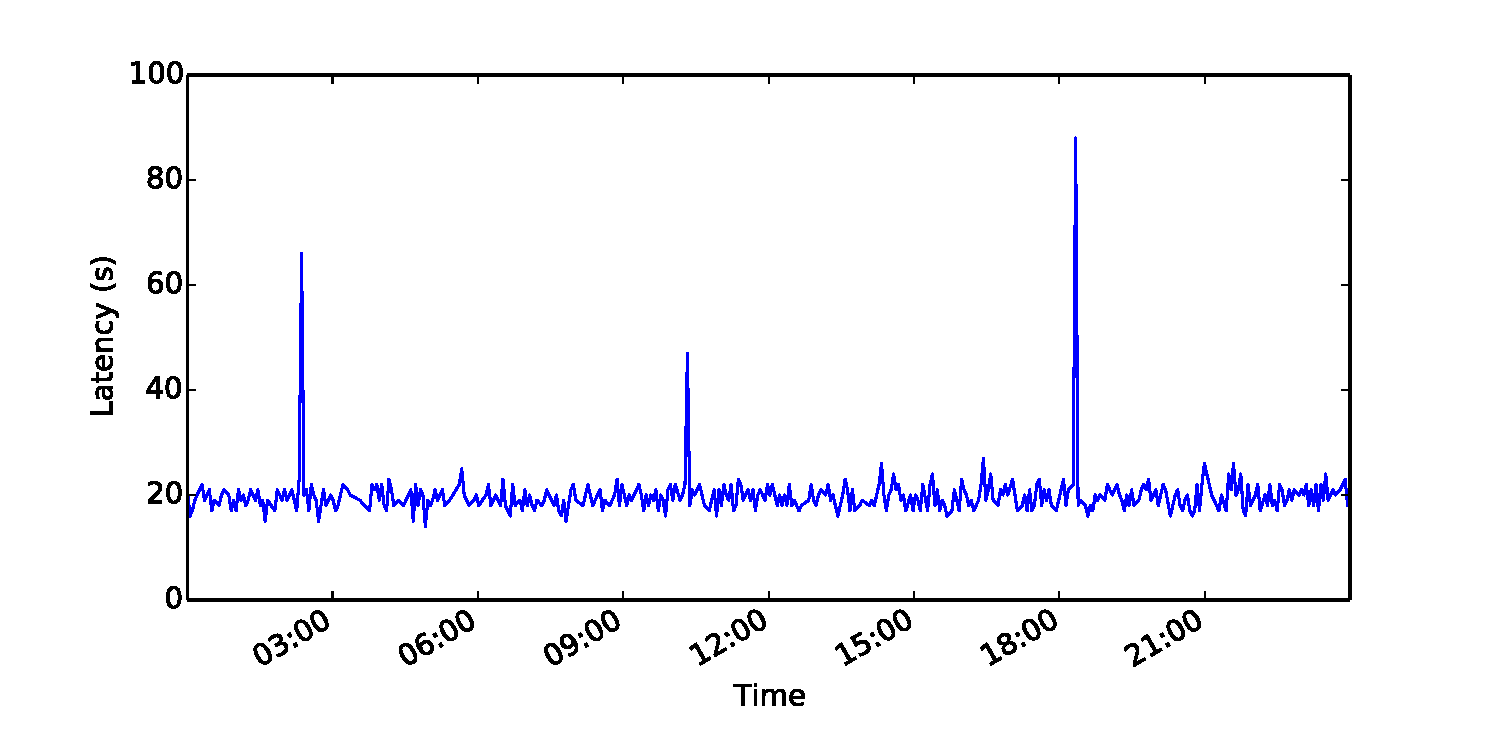
\includegraphics[width=0.85\textwidth]{graphics/online/pnf/pnf_latency_160627.pdf}
 \caption{Typical online Processing and Filtering system latency for a
   24-hour period.  The latency is defined as the time between DAQ event
   time and time when the online filtering processing is complete.  The
   spikes in latency correspond to DAQ run transitions.}
 \label{fig:online_pnf_latency}
\end{figure}

The filter selections used in the online processing and filtering system
have been relatively stable over several years of operation of the
completed IceCube detector, with most seeing only minor updates at the
start of each season.  The majority of physics analyses performed in
IceCube derive from a small set of core filters, while the other filters
are used for more specialized and experimental searches, as well as minimum
bias selections.  These core physics filters include:
\begin{enumerate}
\item Muon track filter searches for high-quality track events from all
  directions that are potentially neutrino-induced tracks.  Up-going events
  for all triggered energies are selected, while only high-energy
  down-going tracks are selected to avoid the large background of
  down-going atmospheric muons at lower energies.  These selected events
  are used as the input to point source and transient neutrino searches.
\item Shower event filter searches for events producing large energy
  depositions in or near the IceCube instrumented volume that are
  potentially neutrino-induced showering events.  These selected events are
  used as the input to searches for high-energy shower events arising from
  atmospheric and astrophysical neutrinos.
\item High charge filter searches for any event depositing a significant
  amount of charge (\textgreater $\sim$1000 photoelectrons) in the IceCube
  instrumented volume.  While having a large overlap with the muon track
  and shower filters at high energies, this filter targets the highest
  energy neutrino events of all types. The selected events are used as
  inputs to searches for high-energy astrophysical and cosmogenic
  neutrinos.
\item Cosmic Ray filters searches for extended air-shower events in IceTop
  station signals.  The selected events are used as inputs to analyses
  targeting the flux, spectrum and composition of the primary cosmic rays
  observed in the Earth's atmosphere.
\item DeepCore contained filter searches for contained, lower-energy
  neutrino events ($\sim10-100 GeV$) from atmospheric neutrino interactions
  that are contained with the more densely instrumented DeepCore region.
  The selected events are used as inputs to analyses that search for
  neutrino oscillation effects.
\end{enumerate}
\subsection{\label{sect:online_jade}Data Handling}

The bulk of South Pole Station data traffic is handled by geosynchronous
satellite links.  Due to the unfavorable location at the South Pole, only
geosynchronous satellites with steeply inclined orbits reach far enough
above the horizon to establish a link.  For a given satellite, this link
provides four to six hours of communications once per sidereal day.
Multiple geosynchronous satellites are currently utilized by the U.S.~
Antarctic Program, providing a $\sim$12-hour window of connectivity with
bandwidth of 1 Mbps or higher.  For the remainder of the day, Iridium
satellites allow limited voice and data connectivity and provide up to 2.4
kbps of bandwidth per connection.

IceCube incorporates Iridium modems into two separate systems.  The IceCube
Teleport System (ITS) uses the Iridium short burst data mode to send short
messages of 1.8 kB or smaller with a typical latency of 30 seconds.
Messages may both originate or terminate at the ITS Iridium modem at the
South Pole.  Messages also contain a recipient ID indicating the intended
host to receive the message, allowing a many-to-many communications
infrastructure between systems running at the South Pole and systems in the
Northern Hemisphere.  The IceCube Messaging System (I3MS) incorporates
multiple Iridium modems and uses the Iridium RUDICS data mode, providing a
2.4 kbit/s bidirectional serial stream per modem and a minimum latency of
$\sim$1.5 seconds.  I3MS runs as a daemon on both ends of the link, accepts
messages via the ZeroMQ distributed messaging protocol, and transports
those messages across the link based on message priority and fair sharing
of bandwidth among all users. I3MS message recipients listen for messages
using ZeroMQ publish-subscribe (PUB-SUB), allowing a given message to be
sent to multiple recipients.

Data handling is provided by three servers running the Java Archival and
Data Exchange (JADE) software (stylized “jade”).  The jade software is a
Java-based reimplementation and expansion of earlier prototype software
called South Pole Archival and Data Exchange (SPADE). The jade software has
four primary tasks: consumption, archival, satellite transmission, and
real-time transmission. The three jade servers operate independently of one
another and each of them are capable of handling the nominal data volume by
itself. Having three servers allows for data handling to continue
seamlessly in case of hardware failure or maintenance.

The jade software is configured with a number of data streams, which
consist of a data server, a dropbox directory, and a filename pattern.  The
data stream dropbox directories are checked on a regular basis for new
files. A file pairing scheme (binary and semaphore) prevents files from
being consumed before they are finished being produced. For each file, a
checksum calculated on the data server is compared to a checksum calculated
on the jade server. This method ensures that the file was copied without
error. After this, the original data file is removed from the data host.

After consumption, files are routed according to the configuration of their
data stream. Files that are too large to send via the satellite link are
archived to a configurable number of archival media copies. The prototype
SPADE software archived to LTO tapes, while the later jade software
archives to large (2+ TB) hard disk drives. All of the archival data is
buffered on the jade server until the archival media is complete. In case
of failure while creating the archival media, all of the files can be
immediately written to fresh archival media with a single command.

Files that are too large to send via the real-time link, but small enough
to send via the satellite link are queued for satellite transmission. The
jade software attempts to bundle multiple files together into 1 GB bundle
archives to allow satellite link operators to manage the daily data
transmission. Very large files ($>$1 GB) are split apart into multiple 1 GB
bundles for the same reason. The jade software will only transfer a
configurable number of bundles to the satellite relay server. If satellite
transmission is not possible, the jade software will buffer the excess
bundles on the jade server, to avoid flooding the relay server
unnecessarily.


Small files ($<$50 KB) with high priority status information are sent via
the real-time link. The real-time link is provided by the I3MS. The jade
software uses JeroMQ, a pure Java implementation of the ZeroMQ protocol, to
connect to I3MS. In cases where the real-time link is not available, I3MS
will queue the messages to be sent when the link becomes available. All
I3MS messages are also sent to jade to send via the satellite link to
ensure delivery if the real-time link should be unavailable for an extended
period of time.

\subsection{\label{sec:online:icecubelive}IceCube Live and Remote Monitoring}

IceCube operations are controlled and monitored centrally by IceCube Live,
a suite of high-level software implemented mostly in the Python programming
language.  IceCube Live consists of two major components: LiveControl,
responsible for controlling data-taking operations and collecting
monitoring data, and the IceCube Live website, responsible for processing
and storing monitoring data as well as presenting this data in webpages and
plots that characterize the state of the IceCube detector.

\subsubsection{LiveControl}

LiveControl executes in the background as a daemon and accepts user input
via XML-RPC.  Operators typically enter commands and check the basic
detector status using a command-line interface.  LiveControl is responsible
for controlling the state of DAQ and online-processing, starting and
stopping data-taking runs, and recording the parameters of these runs.
Standard operation is to request a run start, supplying a configuration
file specifying the DOMs to include in data taking.  LiveControl then
records the run number, configuration, start time, etc. and sends a request
for DAQ to begin data taking.  After data taking commences successfully,
LiveControl waits a specified amount of time, generally eight hours, then
stops the current run and automatically starts a new run using the same
configuration.  This cycle continues until stopped by a user request or a
run fails.  In case of failure, LiveControl attempts to restart data taking
by starting a new run.  Occasionally a hardware failure occurs, and it is
impossible to start a run with the supplied configuration because requested
DOMs are unpowered or temporarily unable to communicate with the IceCube
DAQ.  In this case, LiveControl cycles through predefined partial-detector
configurations in an attempt to exclude problematic DOMs.  This results in
taking data with less than the full number of available strings, but it
greatly reduces the chance of a prolonged complete outage where no IceCube
data is recorded.

A secondary function of LiveControl is the collection, processing, and
forwarding of monitoring data from DAQ, online-processing, and other
components.  Monitoring data consists of a JSON dictionary with a
well-defined format including a creation time, sender name, priority, data
name, and either JSON data or a single integer or floating-point value.
This data is forwarded to LiveControl using ZeroMQ and queued internally
for processing.  A few monitoring quantities indicate serious problems with
the detector, e.g. the online-processing latency is too high.  LiveControl
provides a database of checked monitoring values indexed by service and
data name and raises an alert if the value is out of the specified range or
hasn't been received in a specified amount of time.  The alert usually
includes an email to parties responsible for the affected subsystem and,
for serious problems, triggers an automated page to winterover operators.
Several other types of monitoring data trigger a response by LiveControl.
These include alerts generated internally by subsystems, and such alerts
may trigger emails and pages from LiveControl.  All monitoring data are
forwarded to the IceCube Live website for further processing and display.

\subsubsection{IceCube Live Website}

\begin{table}[!ht]
\begin{tabular}{|c|c|c|c|c|}
\hline Priority & Transport System & Daily Messages & Daily Data & Typical
Latency\\ \hline 1 & ITS (Iridium) & 10,000 & 1 MB & 1 minute \\ \hline 2 &
I3MS (Iridium) & 150,000 & 5 MB & 1--5 minutes \\ \hline 3 & JADE
(Geosynchronous) & 300,000 & 100 MB & 1 day \\ \hline
\end{tabular}
\caption{Statistics for IceCube monitoring messages}
\label{i3messages}
\end{table}

Two operational copies of the IceCube Live website exist: one inside the
IceCube network at the South Pole, and one in the Northern Hemisphere.
Monitoring data reaches the northern website based on priority and using
both geosynchronous and Iridium data transport, summarized in table
\ref{i3messages}.

Messages reaching the website are processed by the DBServer daemon and
inserted into one of several database tables depending on content.
Messages also may contain directives requesting DBServer to send email, by
specifying email recipients and content, or requesting that the monitoring
message be published using ZeroMQ PUB-SUB, allowing the message to be
passed to an external process.  The IceCube Live website itself uses the
Django framework and contains pages that create sophisticated views of
monitoring data stored in the database.  These pages include a front page
displaying active alerts and plots of event rates and processing latencies
from the previous few hours, and a page for each run that displays start
time, stop time, and other essential data.  The run page contains low-level
diagnostic data that includes e.g. charge histograms, digitizer baselines,
and occupancy for each DOM, and is used to diagnose problems with detector
components that occurred during the run and to determine if the run can be
used in physics analysis.

Finally, the IceCube Live website in the Northern Hemisphere transmits
messages to LiveControl using ITS and I3MS.  This capability is used to
retransmit messages sent using the Slack chat service to the South Pole,
allowing the IceCube winterover operators to chat with experts in the
Northern Hemisphere during periods with no geosynchronous satellite
connectivity.  This connection also provides a limited capability to
control the detector, for example allowing operators in the north to
remotely issue HitSpool requests.



\subsection{Operational Performance}

Full detector operational uptime is highly valued. Many redundancies and
fail-safes have been implemented to achieve an average uptime of greater
than 99\,\%. Each computing hub and server is equipped with redundant power
supplies which are buffered with redundant UPSs. The UPS backup battery
power allows the detector to remain fully operational for 25 minutes in the
event of an AC power outage.

The Nagios systems monitoring software is incorporated into all IceCube
subsystems and communicates with IceCube LiveControl. In the event of
predefined detector failure modes, alerts are sent via email and in more
urgent scenarios the Winter Overs are paged via hand-held radio. Detector
data taking is automatically restarted with an alternate or partial
detector run configuration in the event of component failure.  This
automation maintains as large a fraction of the detector operational as
possible.

%\begin{figure}[!h]
% \centering
% 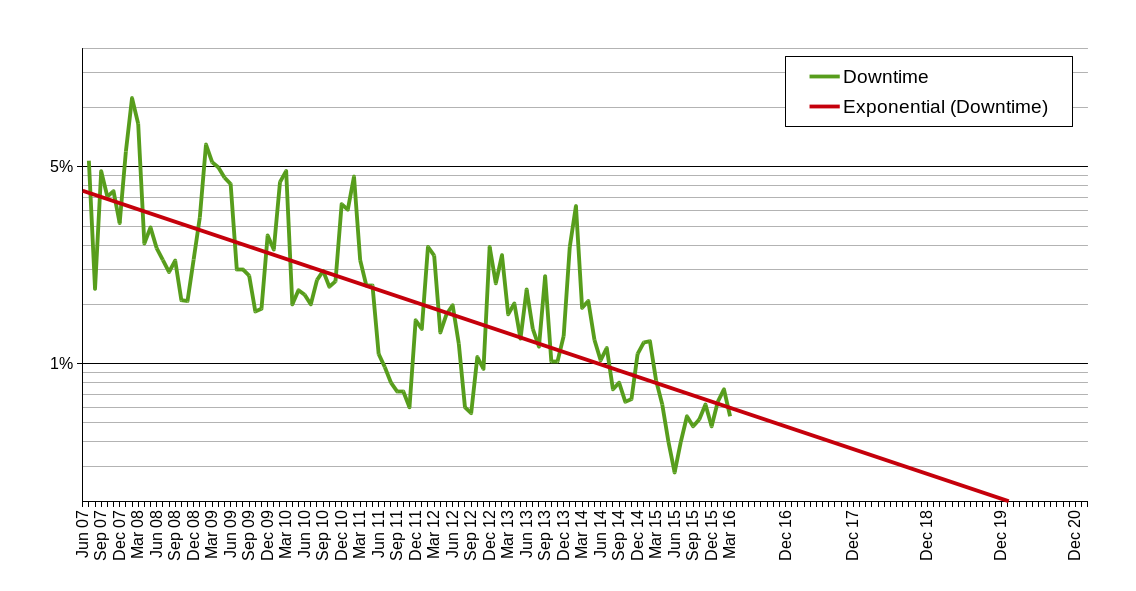
\includegraphics[width=0.8\textwidth]{graphics/uptime/downtime.png}
% \caption{Downtime of the IceCube detector.}
% \label{fig:downtime}
%\end{figure}

The recovery of data from all but the last few minutes of runs that fail,
and the recent implementation of continuous data-taking, have improved
detector stability and decreased detector downtime. These features
contribute to an average “clean uptime” of around 97-98\,\% of
full-detector, analysis-ready data. We are now regularly exceeding our
target clean uptime of 95\,\%.

\begin{figure}[!h]
 \centering
 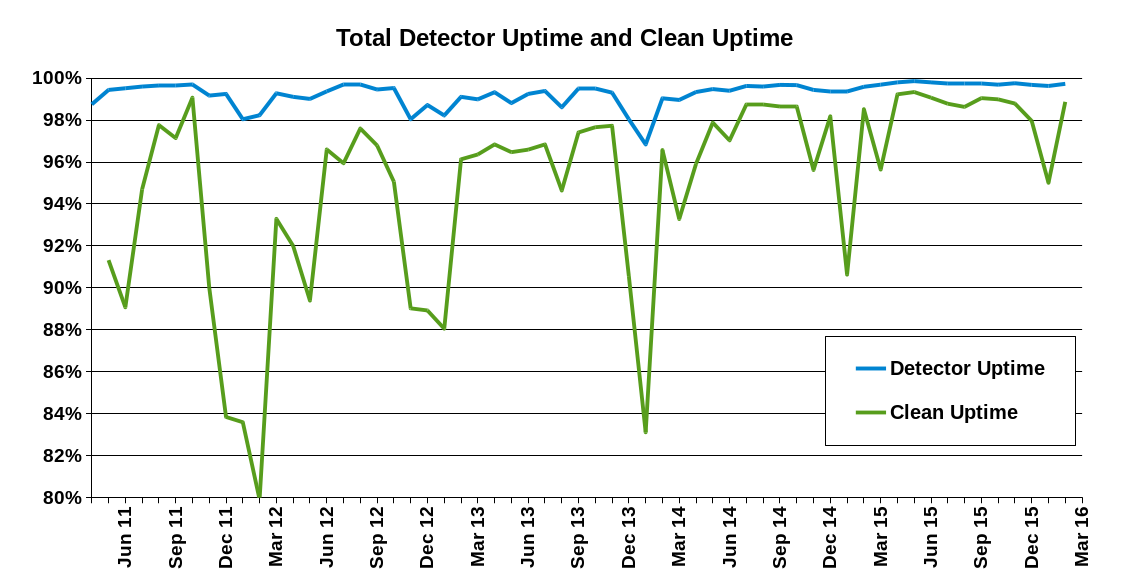
\includegraphics[width=0.8\textwidth]{graphics/uptime/clean-uptime.png}
 \caption{Uptime of the IceCube detector since IC86-2011.}
 \label{fig:clean-uptime}
\end{figure}

About 0.2\,\% of the loss in clean uptime is due to the failed portions of
runs that are not usable for analysis. There is around 1\,\% of clean
uptime loss due to runs not using the full-detector configuration. This
occurs when certain components of the detector are excluded from the run
configuration during required repairs and maintenance. This data is still
good for analyses that have less strict requirements on the active detector
volume. There is approximately a 1\,\% loss of clean uptime due to
maintenance, commissioning, and verification runs, and short runs that are
less than 10 minutes in duration. The experiment control system and DAQ
have recently implemented 32-hour periods of continuous data-taking. This
new feature has eliminated approximately 90–120 seconds of downtime between
each run transition, gaining roughly 0.5\,\% of uptime.

\begin{figure}[!h]
	\centering
    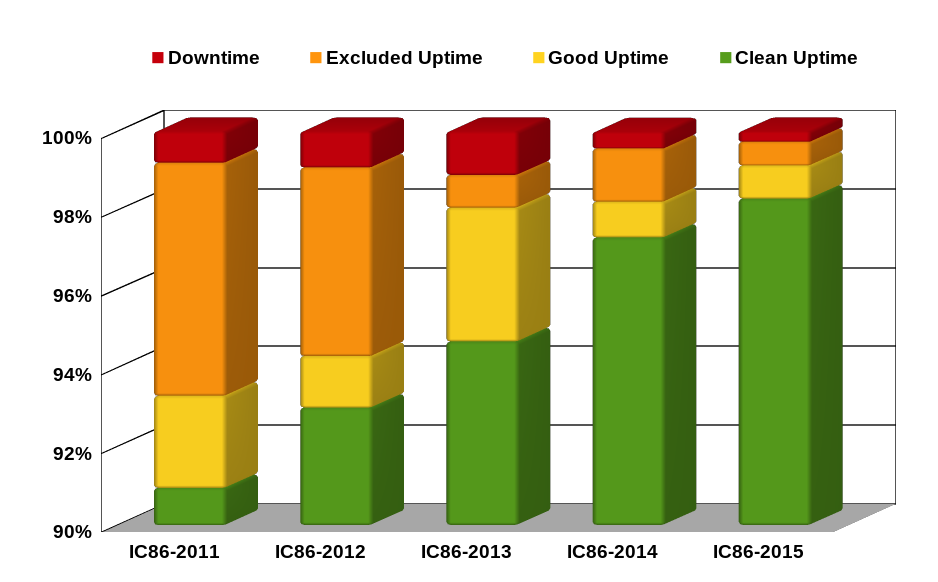
\includegraphics[width=0.8\textwidth]{graphics/uptime/bar-chart.png}
	\caption{Detector performance by run period.}
	\label{fig:period-performace}
\end{figure}


